\section{Strain Analysis and Discussion}
 
\graphicspath{{Chapter4/Figs/}}

\begin{frame}
 \frametitle{Strain Analysis}
 \framesubtitle{}
 \label{ch4:}
 
  Model parameters for Shen algorithm
  
  Data Set: CNRS Solution - MIDAS
  \begin{itemize}
    \item Wt=6
    \item dmin = 1km
    \item dmax = 500km
    \item dstep = 1km
    \item ltype = gaussian
    \item x step = y step = 0.5 $^{\circ}$
    \item \underline{region boundaries}
    
    \textbf{Greece:} east: 18$^{\circ}$, west: 30$^{\circ}$, south: 34$^{\circ}$, north: 43$^{\circ}$
    
    \textbf{Italy:} east: 4$^{\circ}$, west: 18$^{\circ}$, south: 32$^{\circ}$, north: 48$^{\circ}$
  \end{itemize}

\end{frame}
\note{}

\begin{frame}
  \frametitle{Strain Analysis}
  \framesubtitle{Greece region}
  \label{ch4:}
   
  \begin{columns}
    \begin{column}{0.5\textwidth}
      \begin{center}
        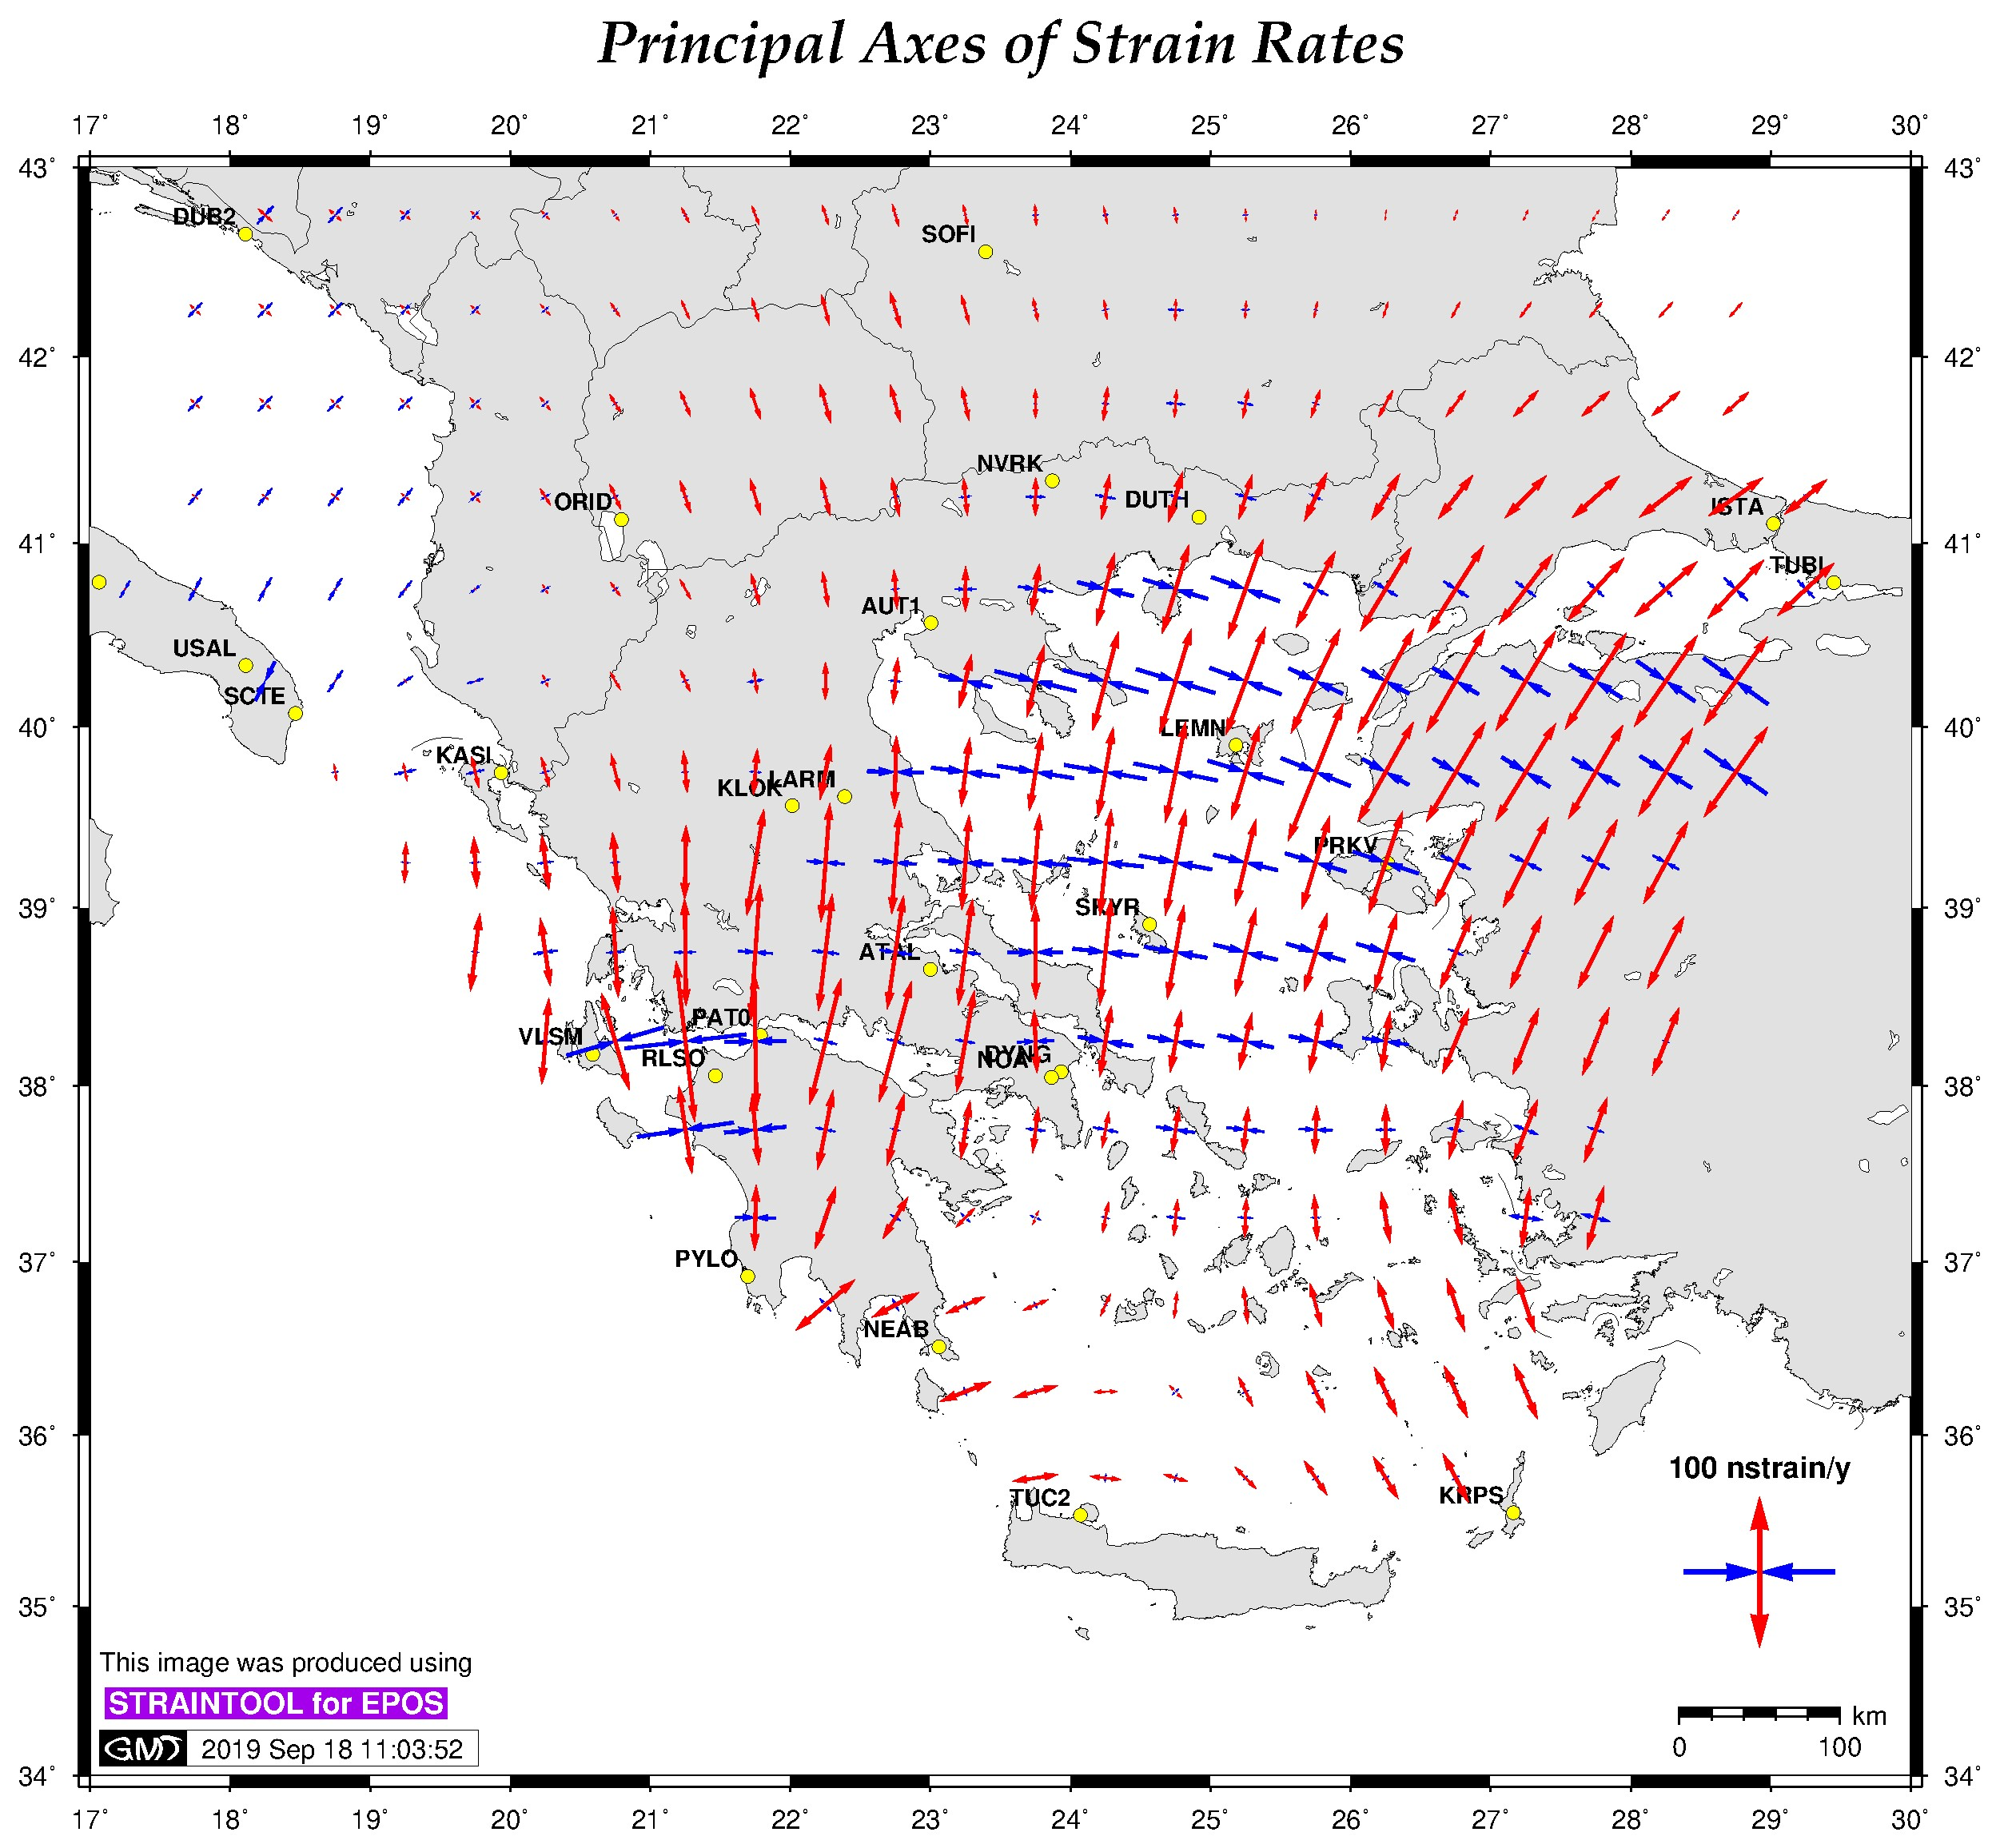
\includegraphics[width=.98\textwidth]{grmidas-output_str.jpg}   
      \end{center}
    \end{column}
    \begin{column}{0.5\textwidth}
      \begin{center}
        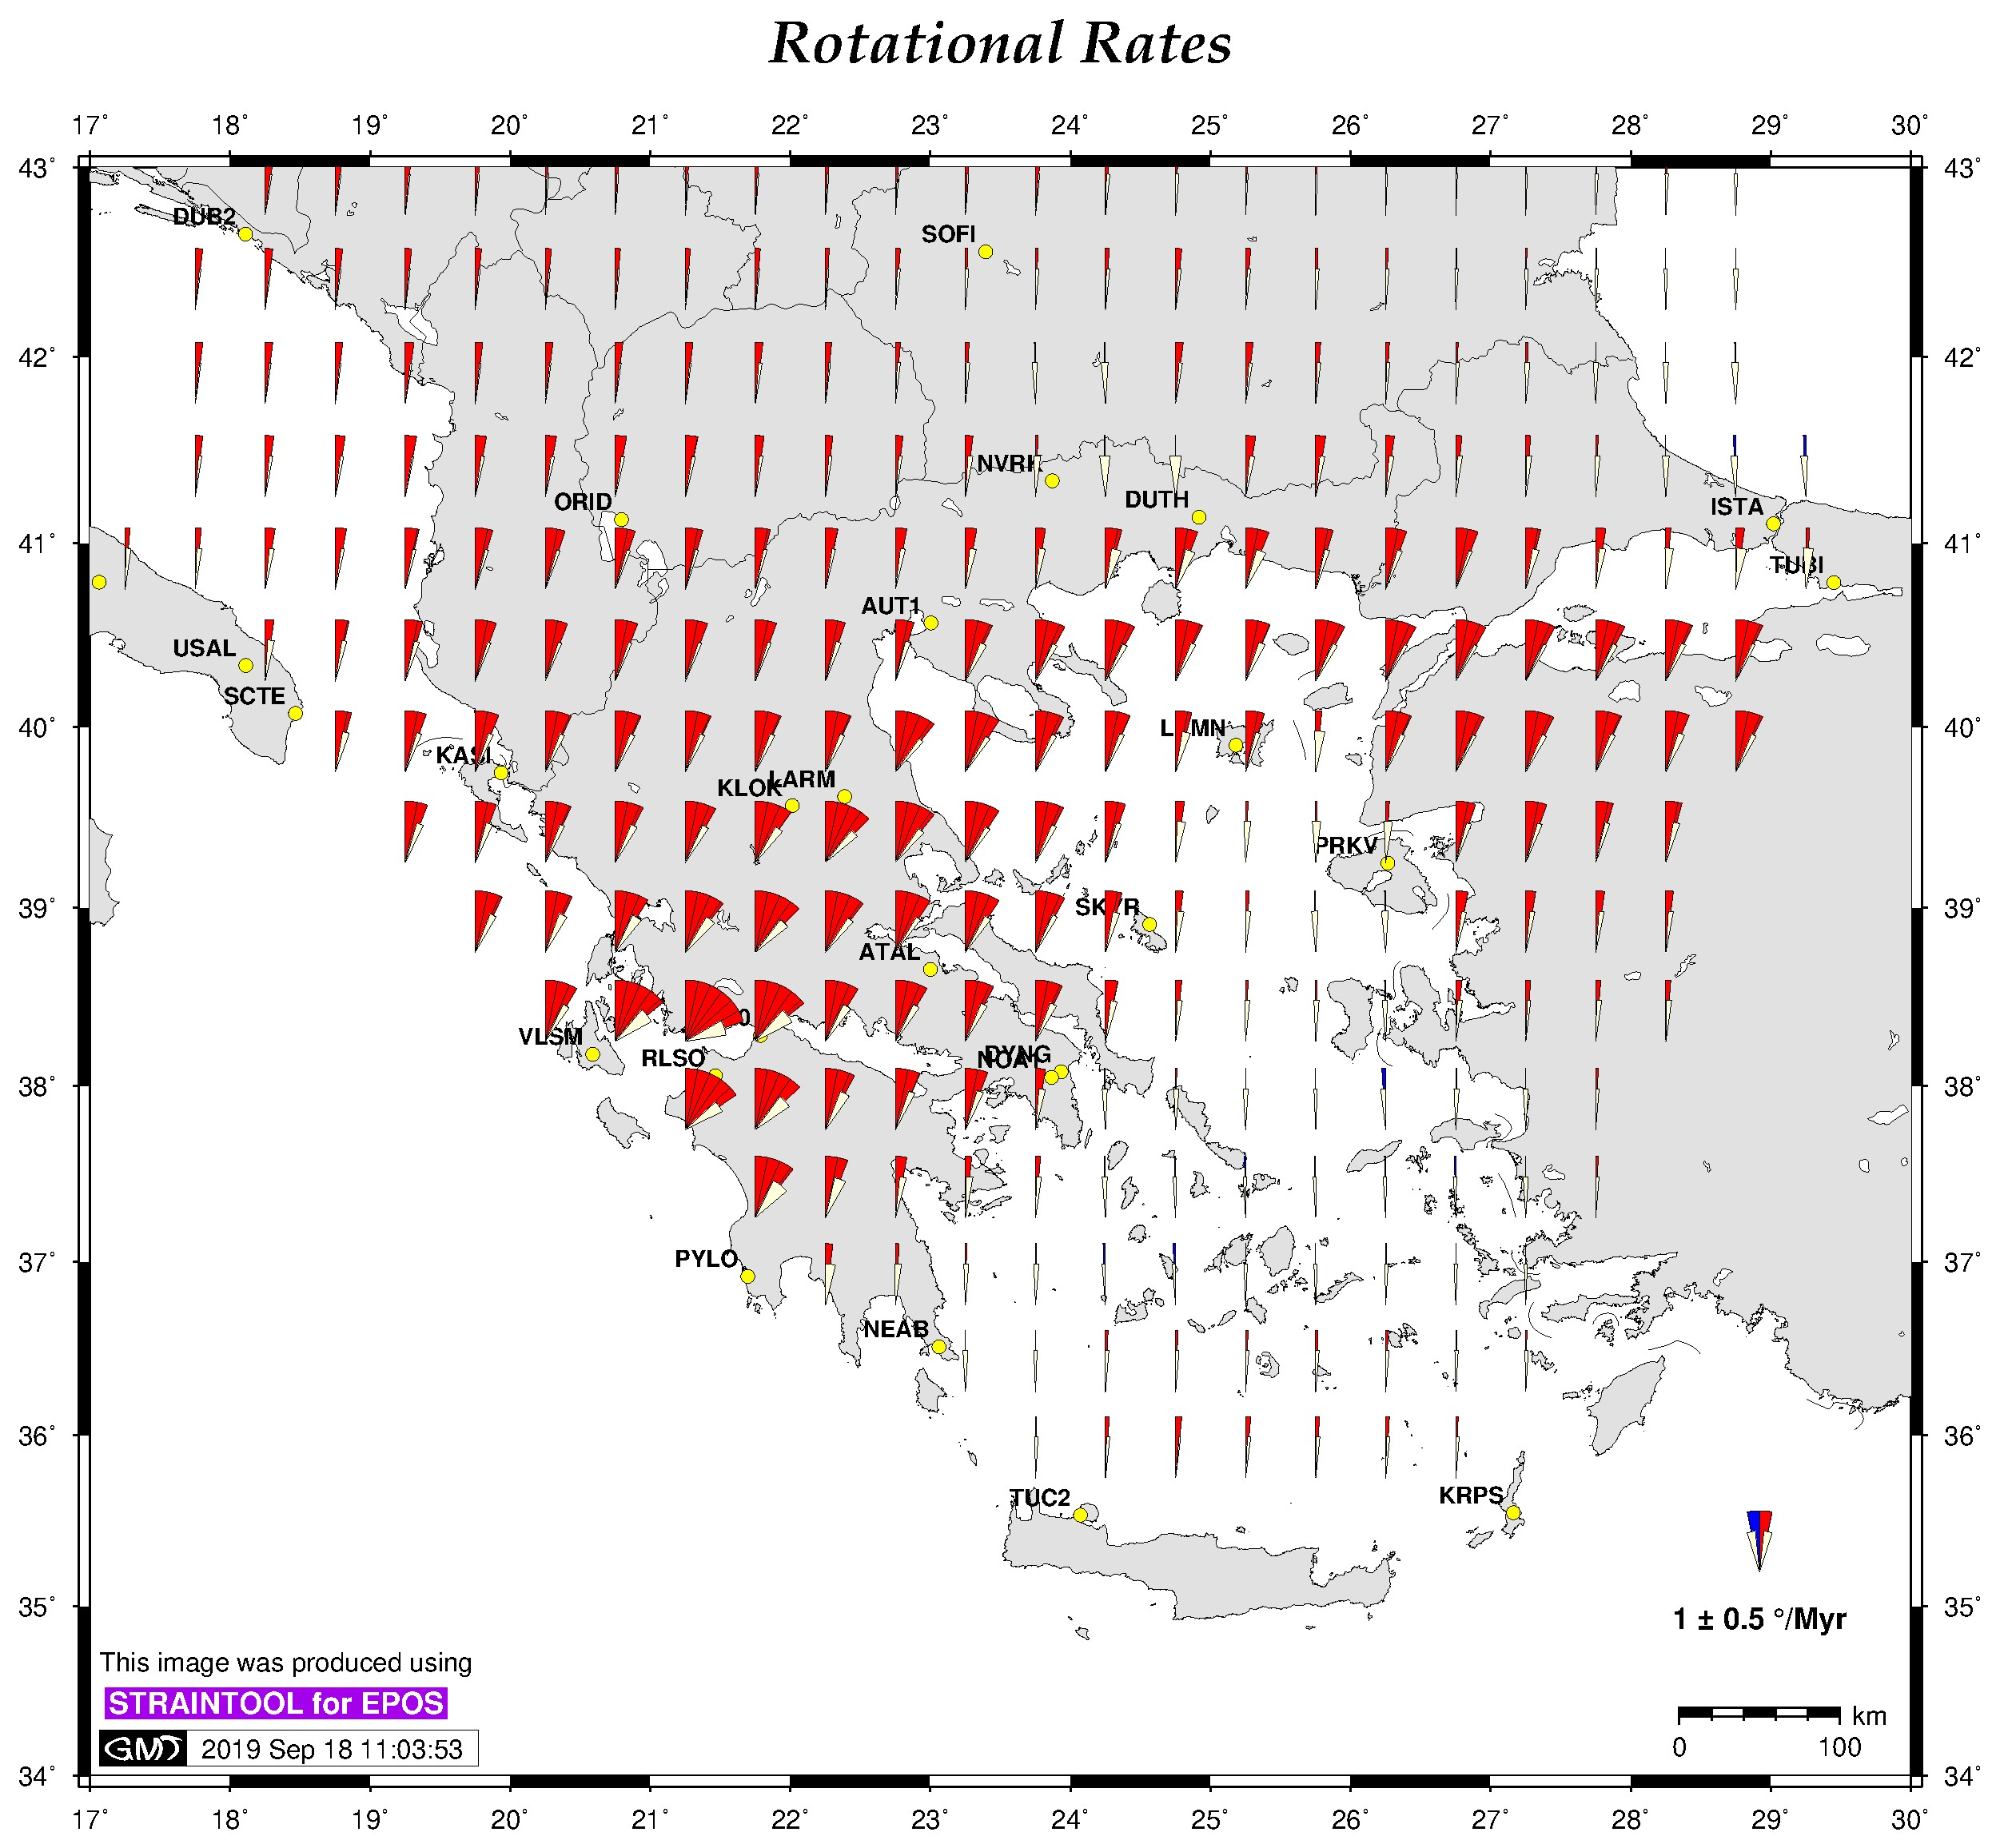
\includegraphics[width=0.98\textwidth]{grmidas-output_rot.jpg}     
      \end{center}
    \end{column}
  \end{columns}

\end{frame}
\note{}

\begin{frame}
 \frametitle{Product Validation}
 \framesubtitle{Greece region}
 \label{ch4:}
   
  \begin{columns}
    \begin{column}{0.5\textwidth}
      \begin{center}
        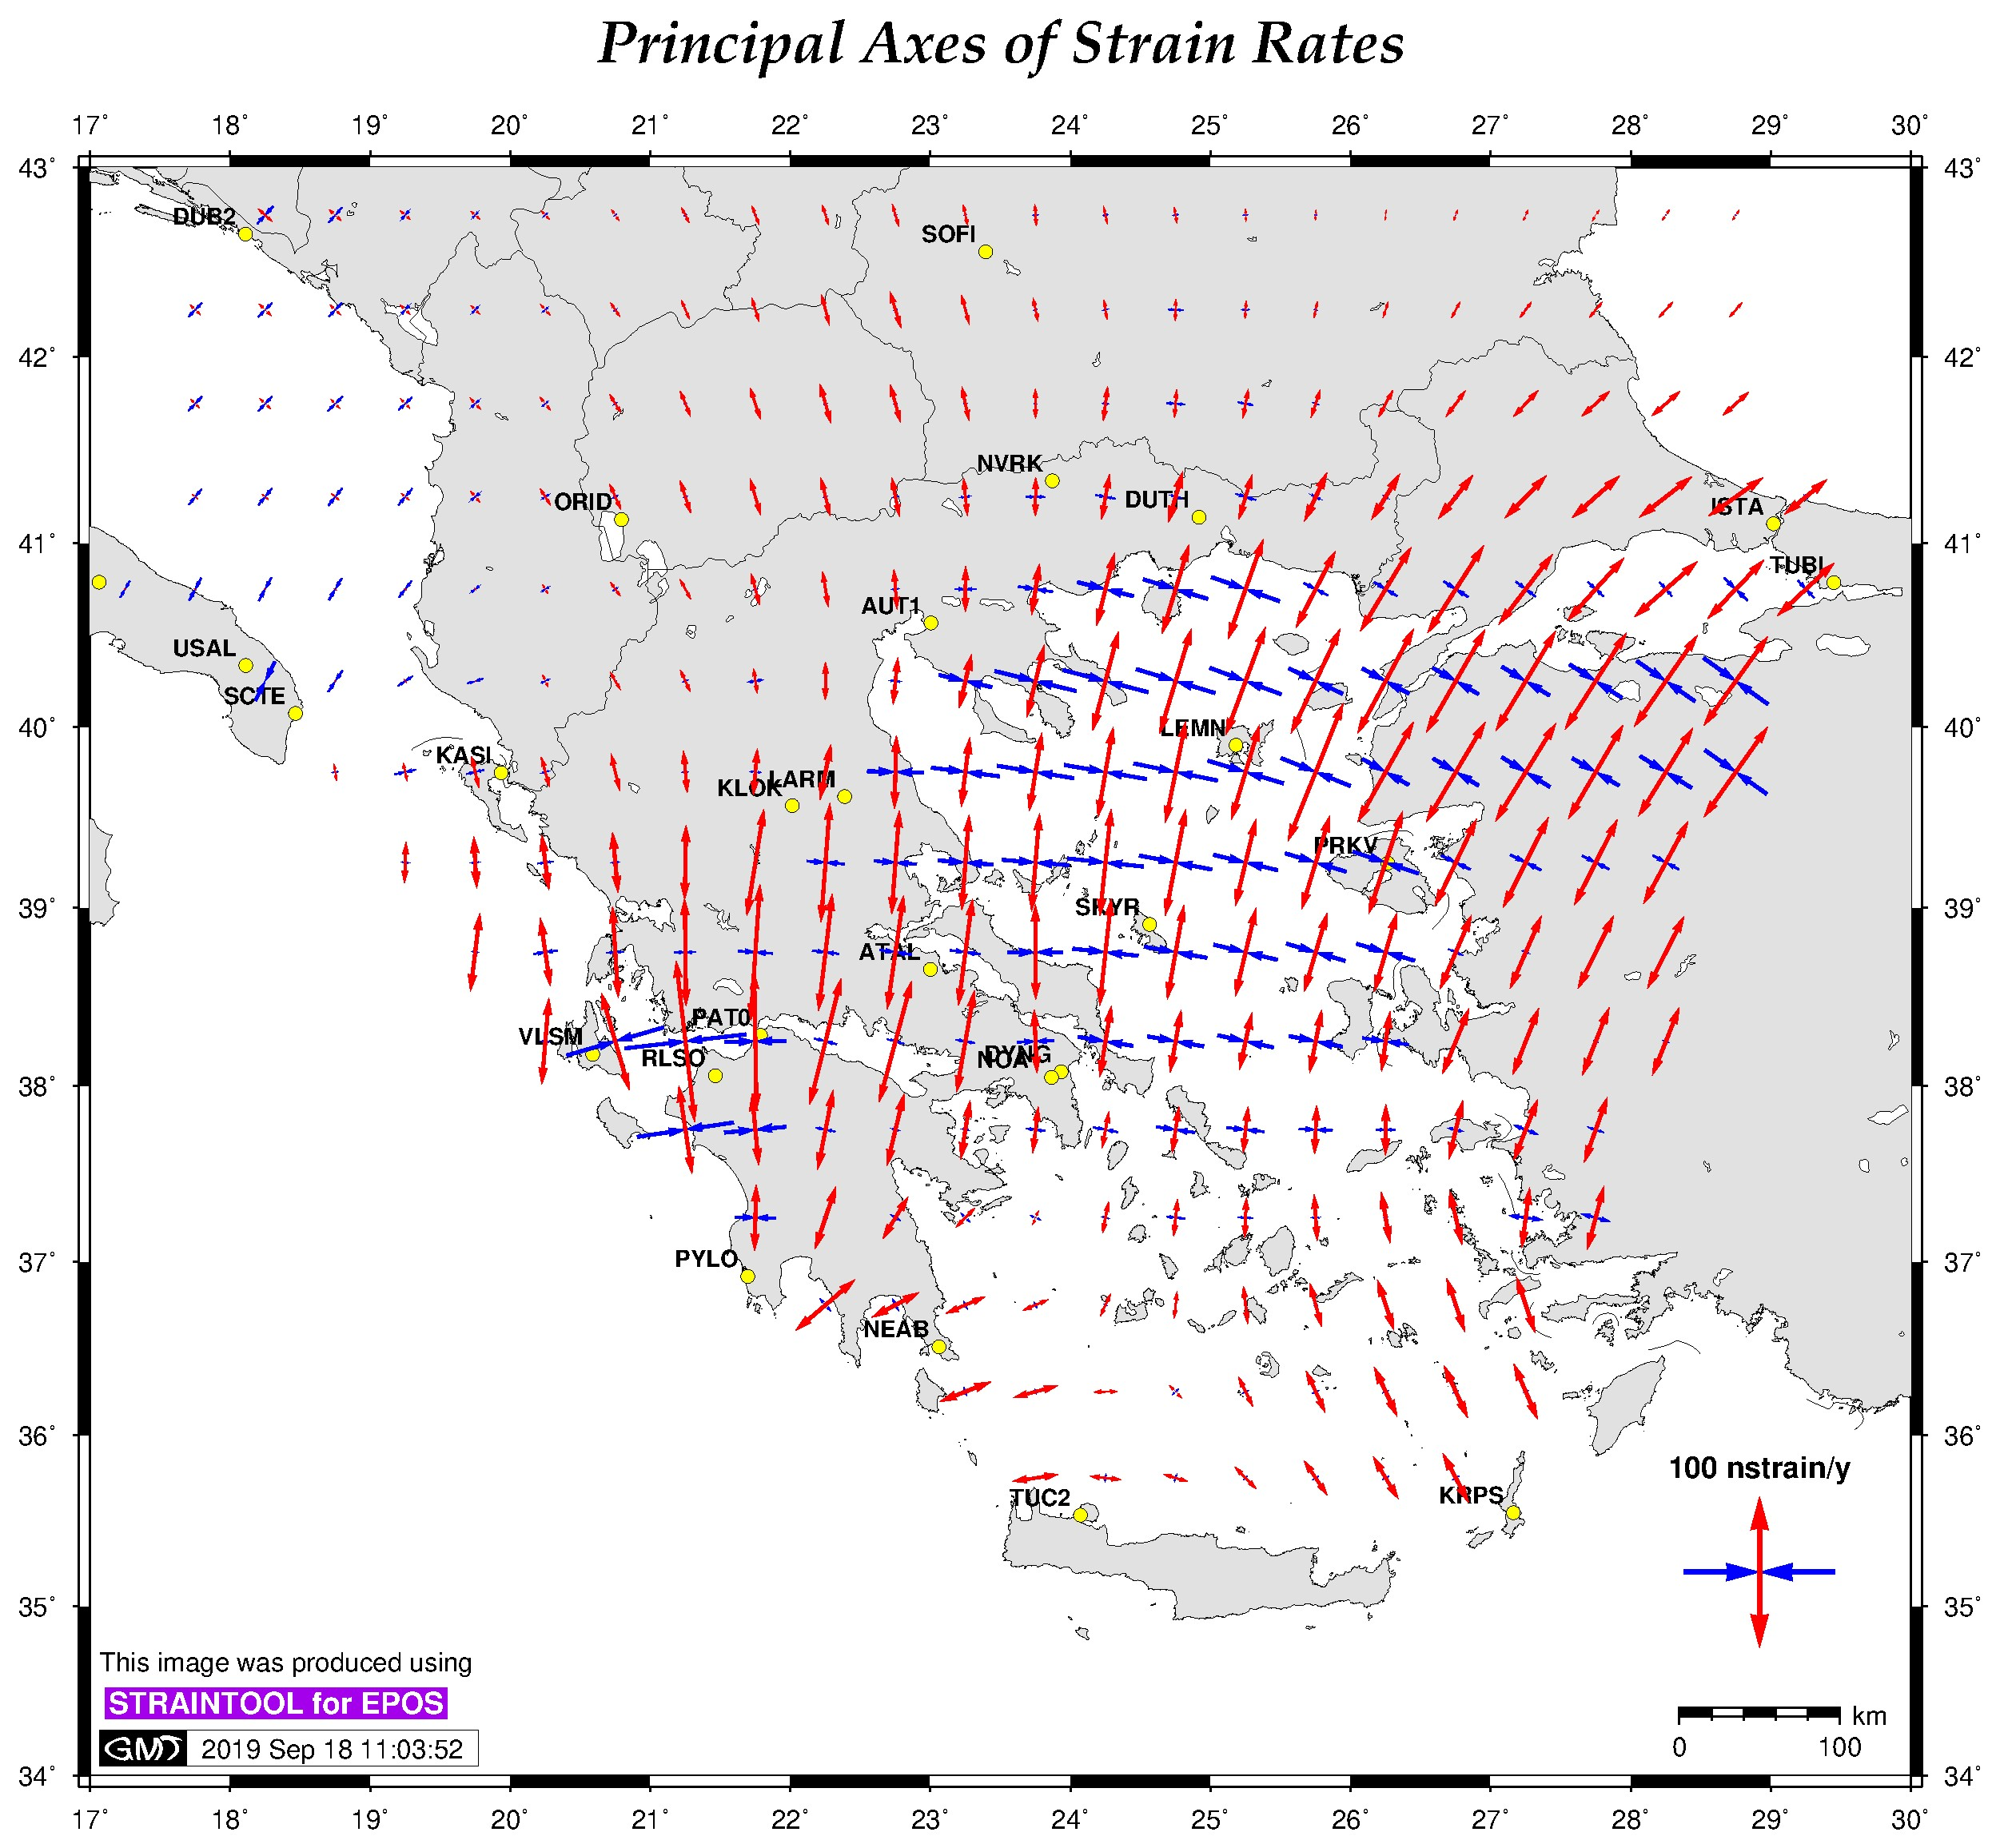
\includegraphics[width=.98\textwidth]{grmidas-output_str.jpg}
      \end{center}
    \end{column}
    \begin{column}{0.5\textwidth}
      \begin{center}
        \citet{Floyd2010}
        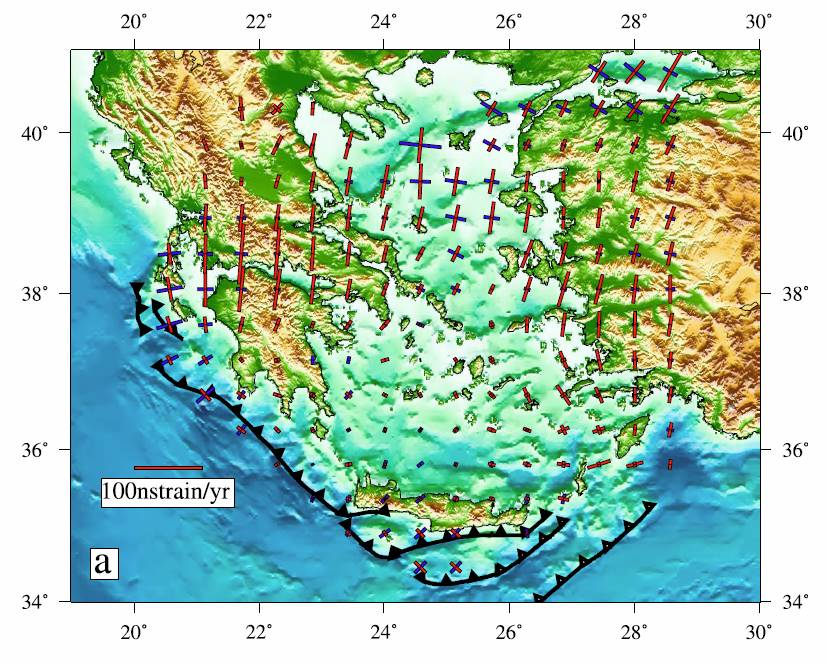
\includegraphics[width=0.98\textwidth]{floyd_greece.jpg}     
      \end{center}
    \end{column}
  \end{columns}

\end{frame}
\note{}

\begin{frame}
  \frametitle{Strain Analysis}
  \framesubtitle{Greece region}
  \label{ch4:}
  \begin{columns}
    \begin{column}{0.5\textwidth}
      \begin{center}
        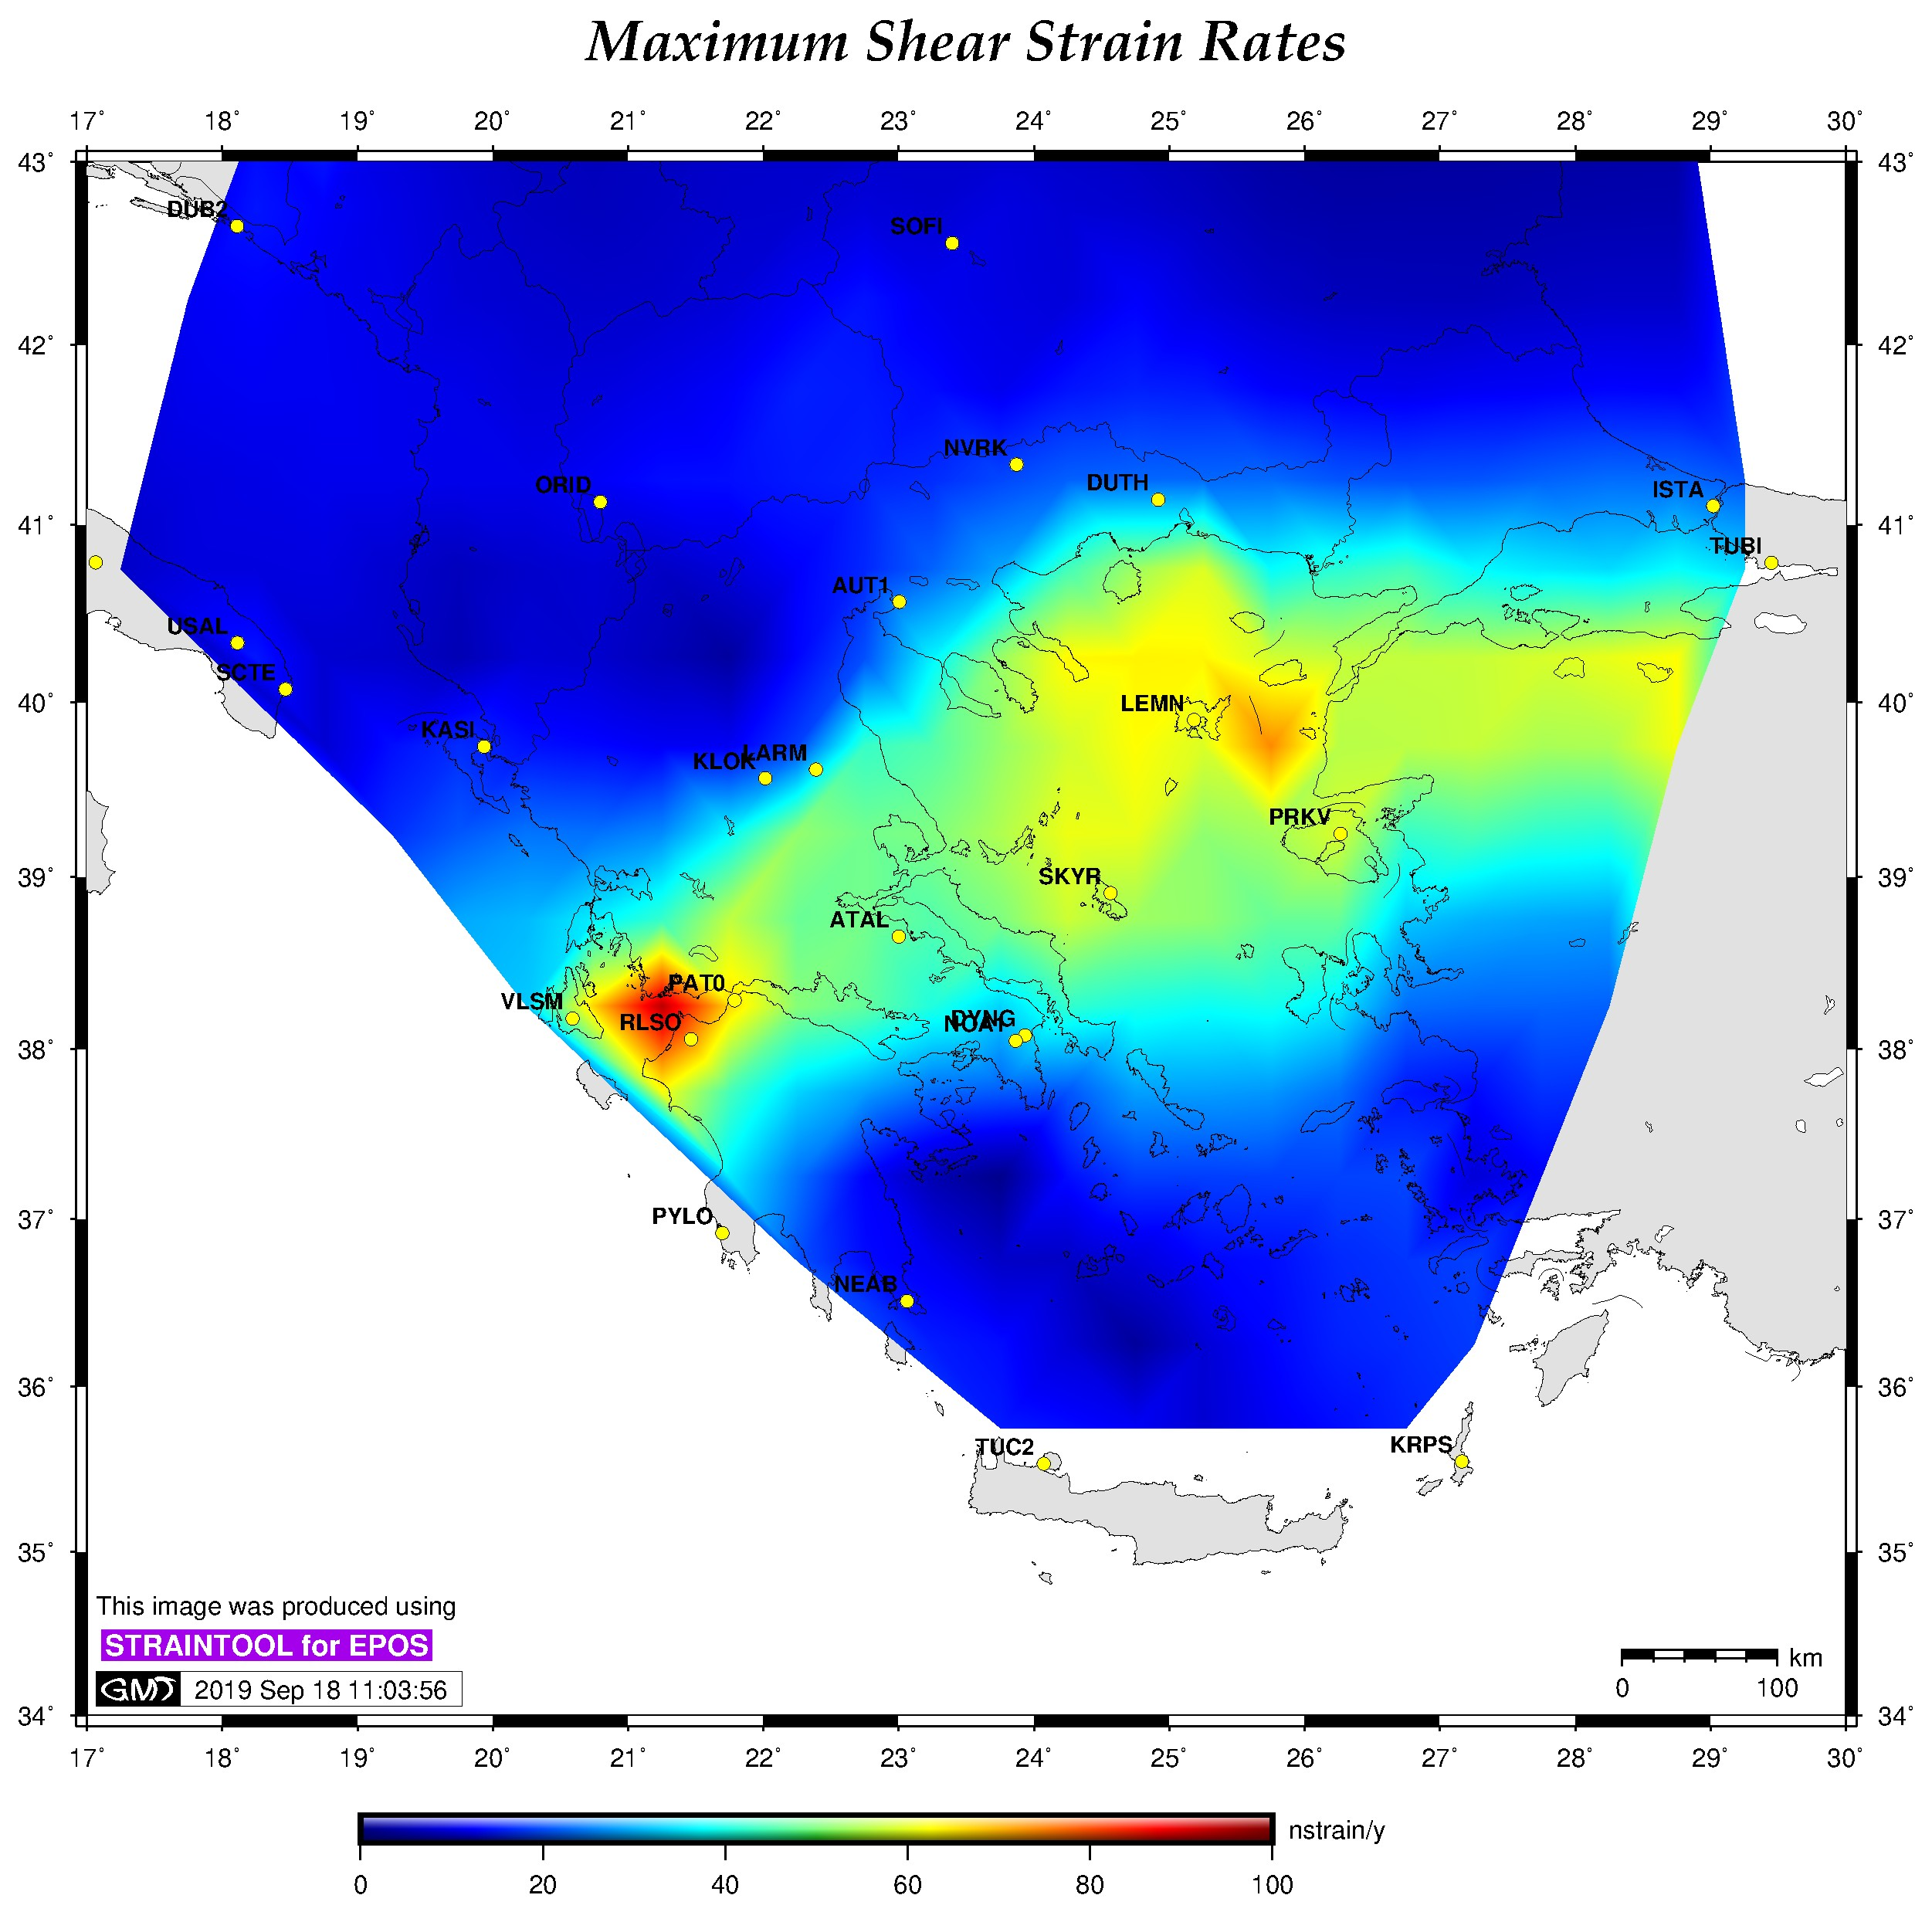
\includegraphics[width=.98\textwidth]{grmidas-output_gtot.jpg}   
      \end{center}
    \end{column}
    \begin{column}{0.5\textwidth}
      \begin{center}
        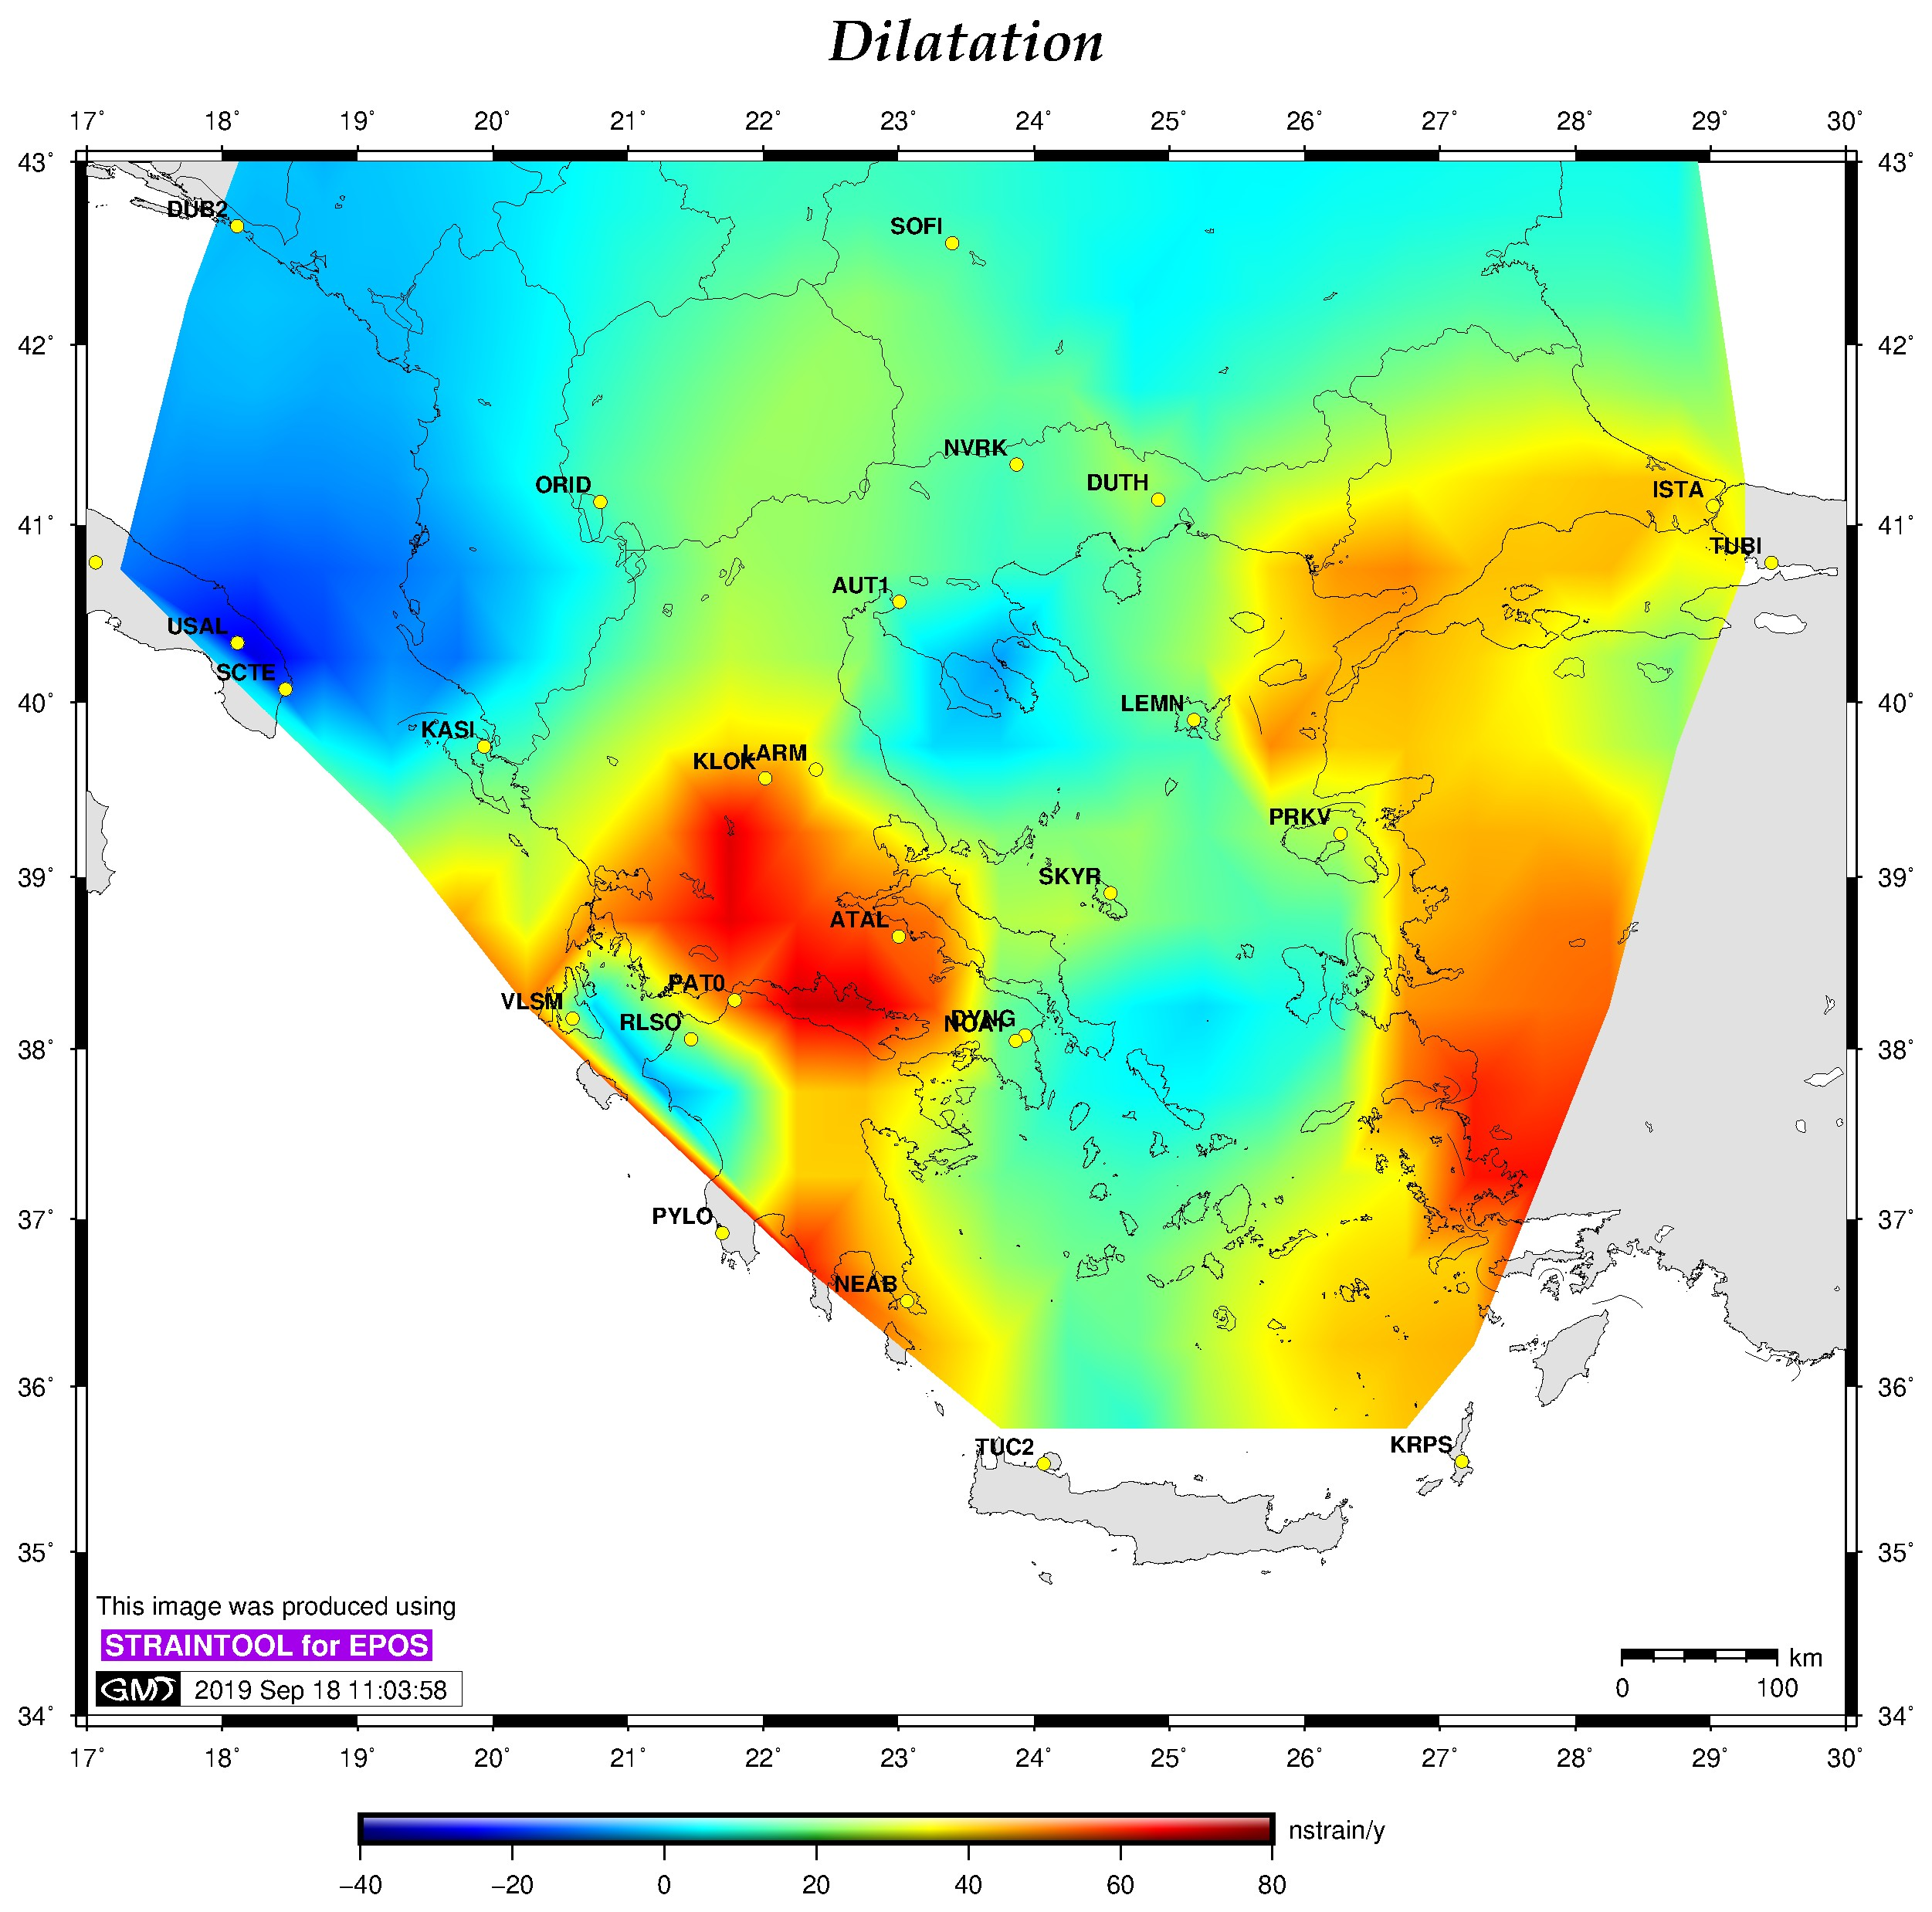
\includegraphics[width=0.98\textwidth]{grmidas-output_dil.jpg}     
      \end{center}
    \end{column}
  
  \end{columns}

\end{frame}
\note{}


\begin{frame}
  \frametitle{Strain Analysis}
  \framesubtitle{Italy region}
  \label{ch4:}
  \begin{columns}
    \begin{column}{0.5\textwidth}
      \begin{center}
        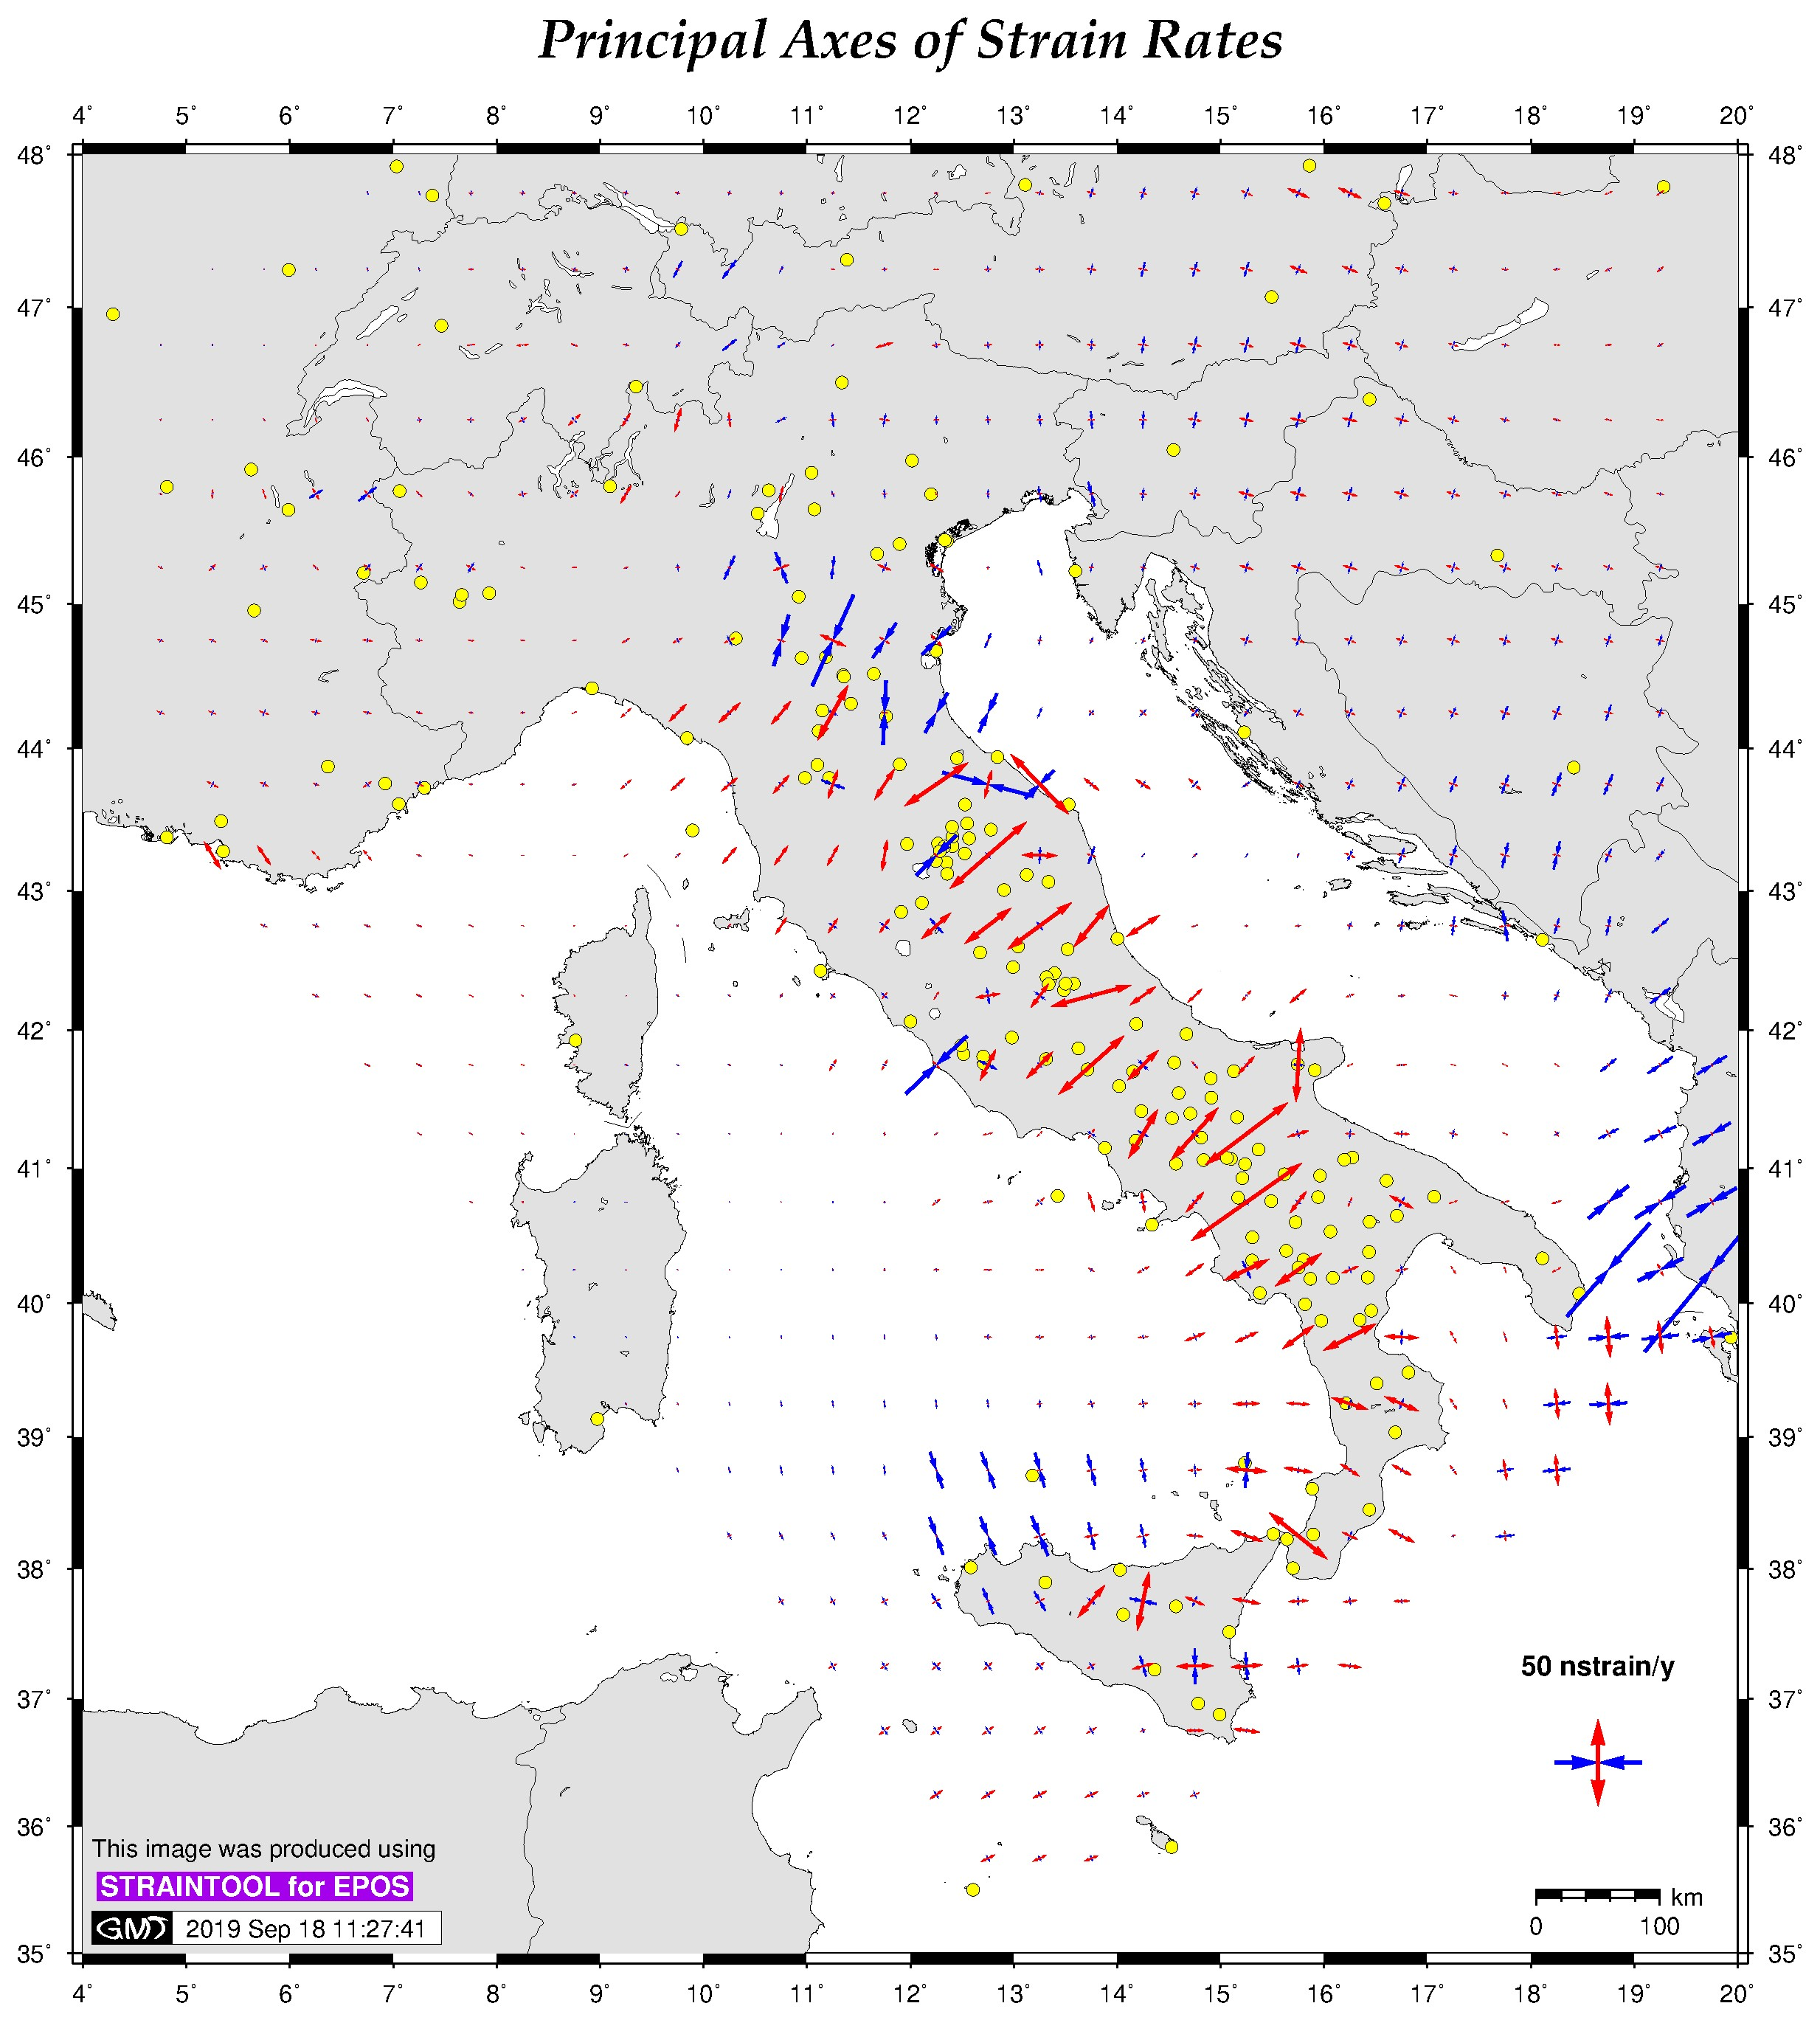
\includegraphics[width=.98\textwidth]{itmidas-output_str.jpg}   
      \end{center}
    \end{column}
    \begin{column}{0.5\textwidth}
      \begin{center}
        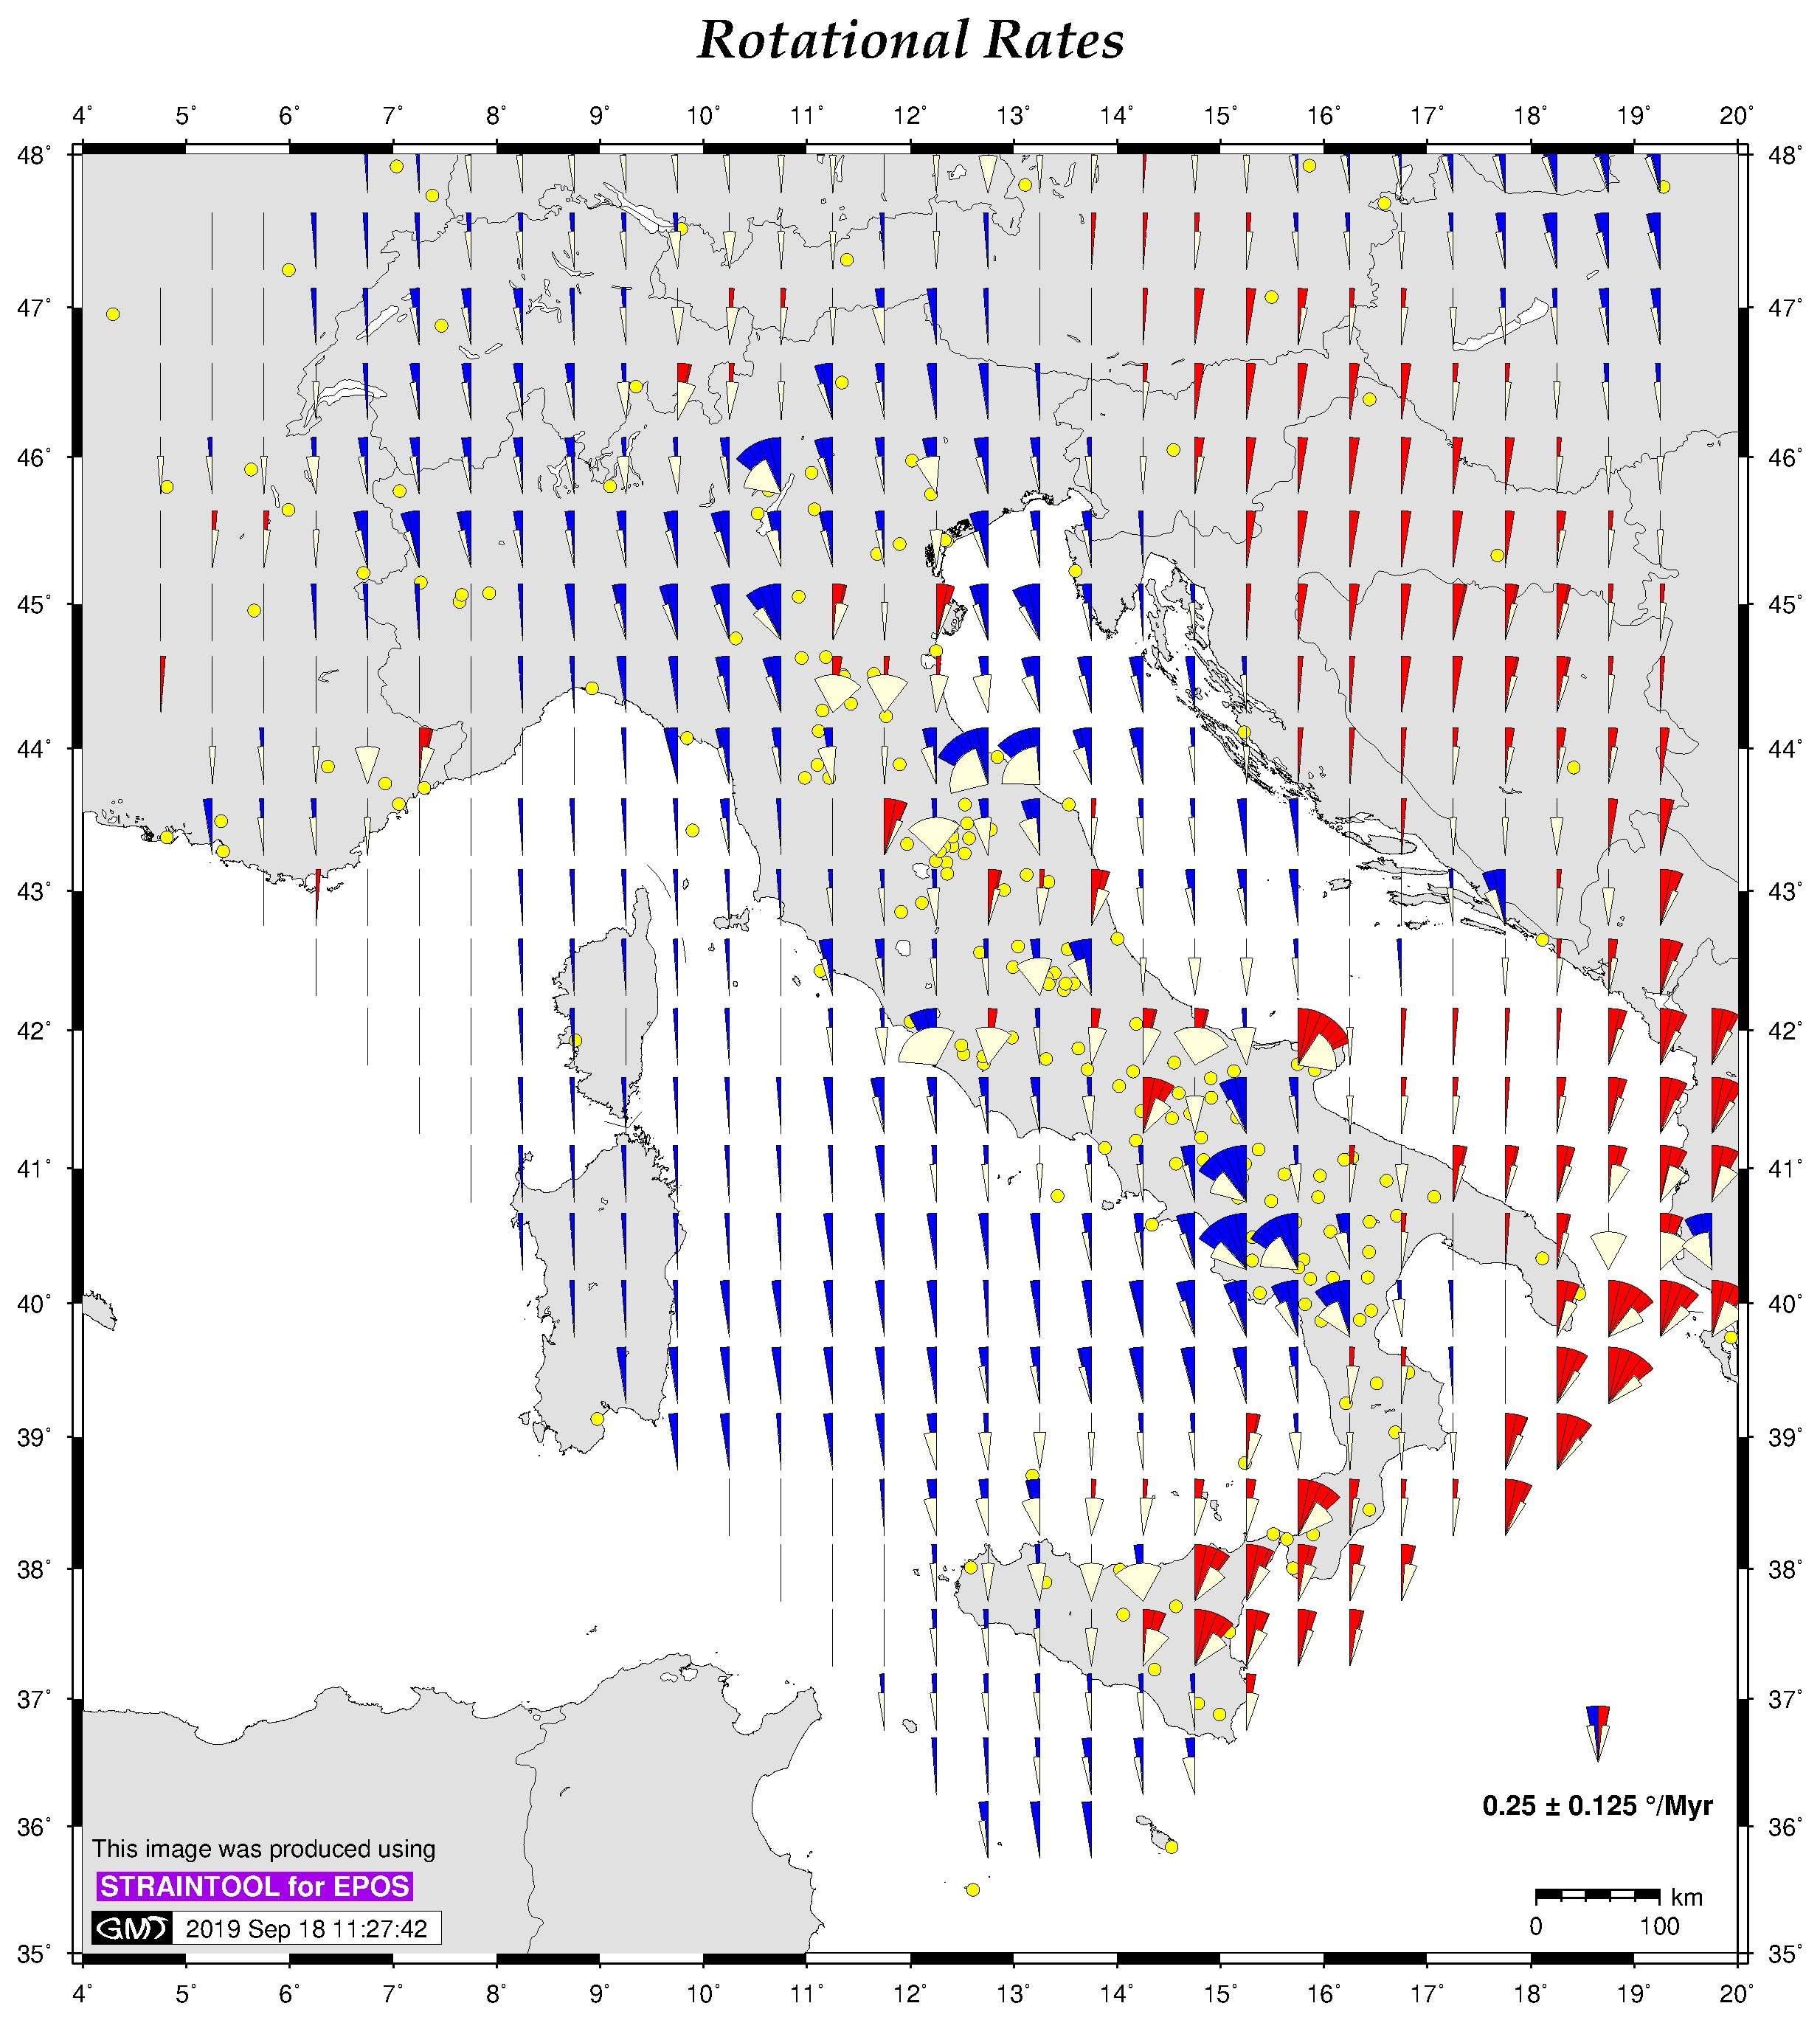
\includegraphics[width=0.98\textwidth]{itmidas-output_rot.jpg}     
      \end{center}
    \end{column}
  \end{columns}

\end{frame}
\note{}

\begin{frame}
  \frametitle{Product Validation}
  \framesubtitle{Italy region}
  \label{ch4:}

  \begin{columns}
    \begin{column}{0.4\textwidth}
      \begin{center}
        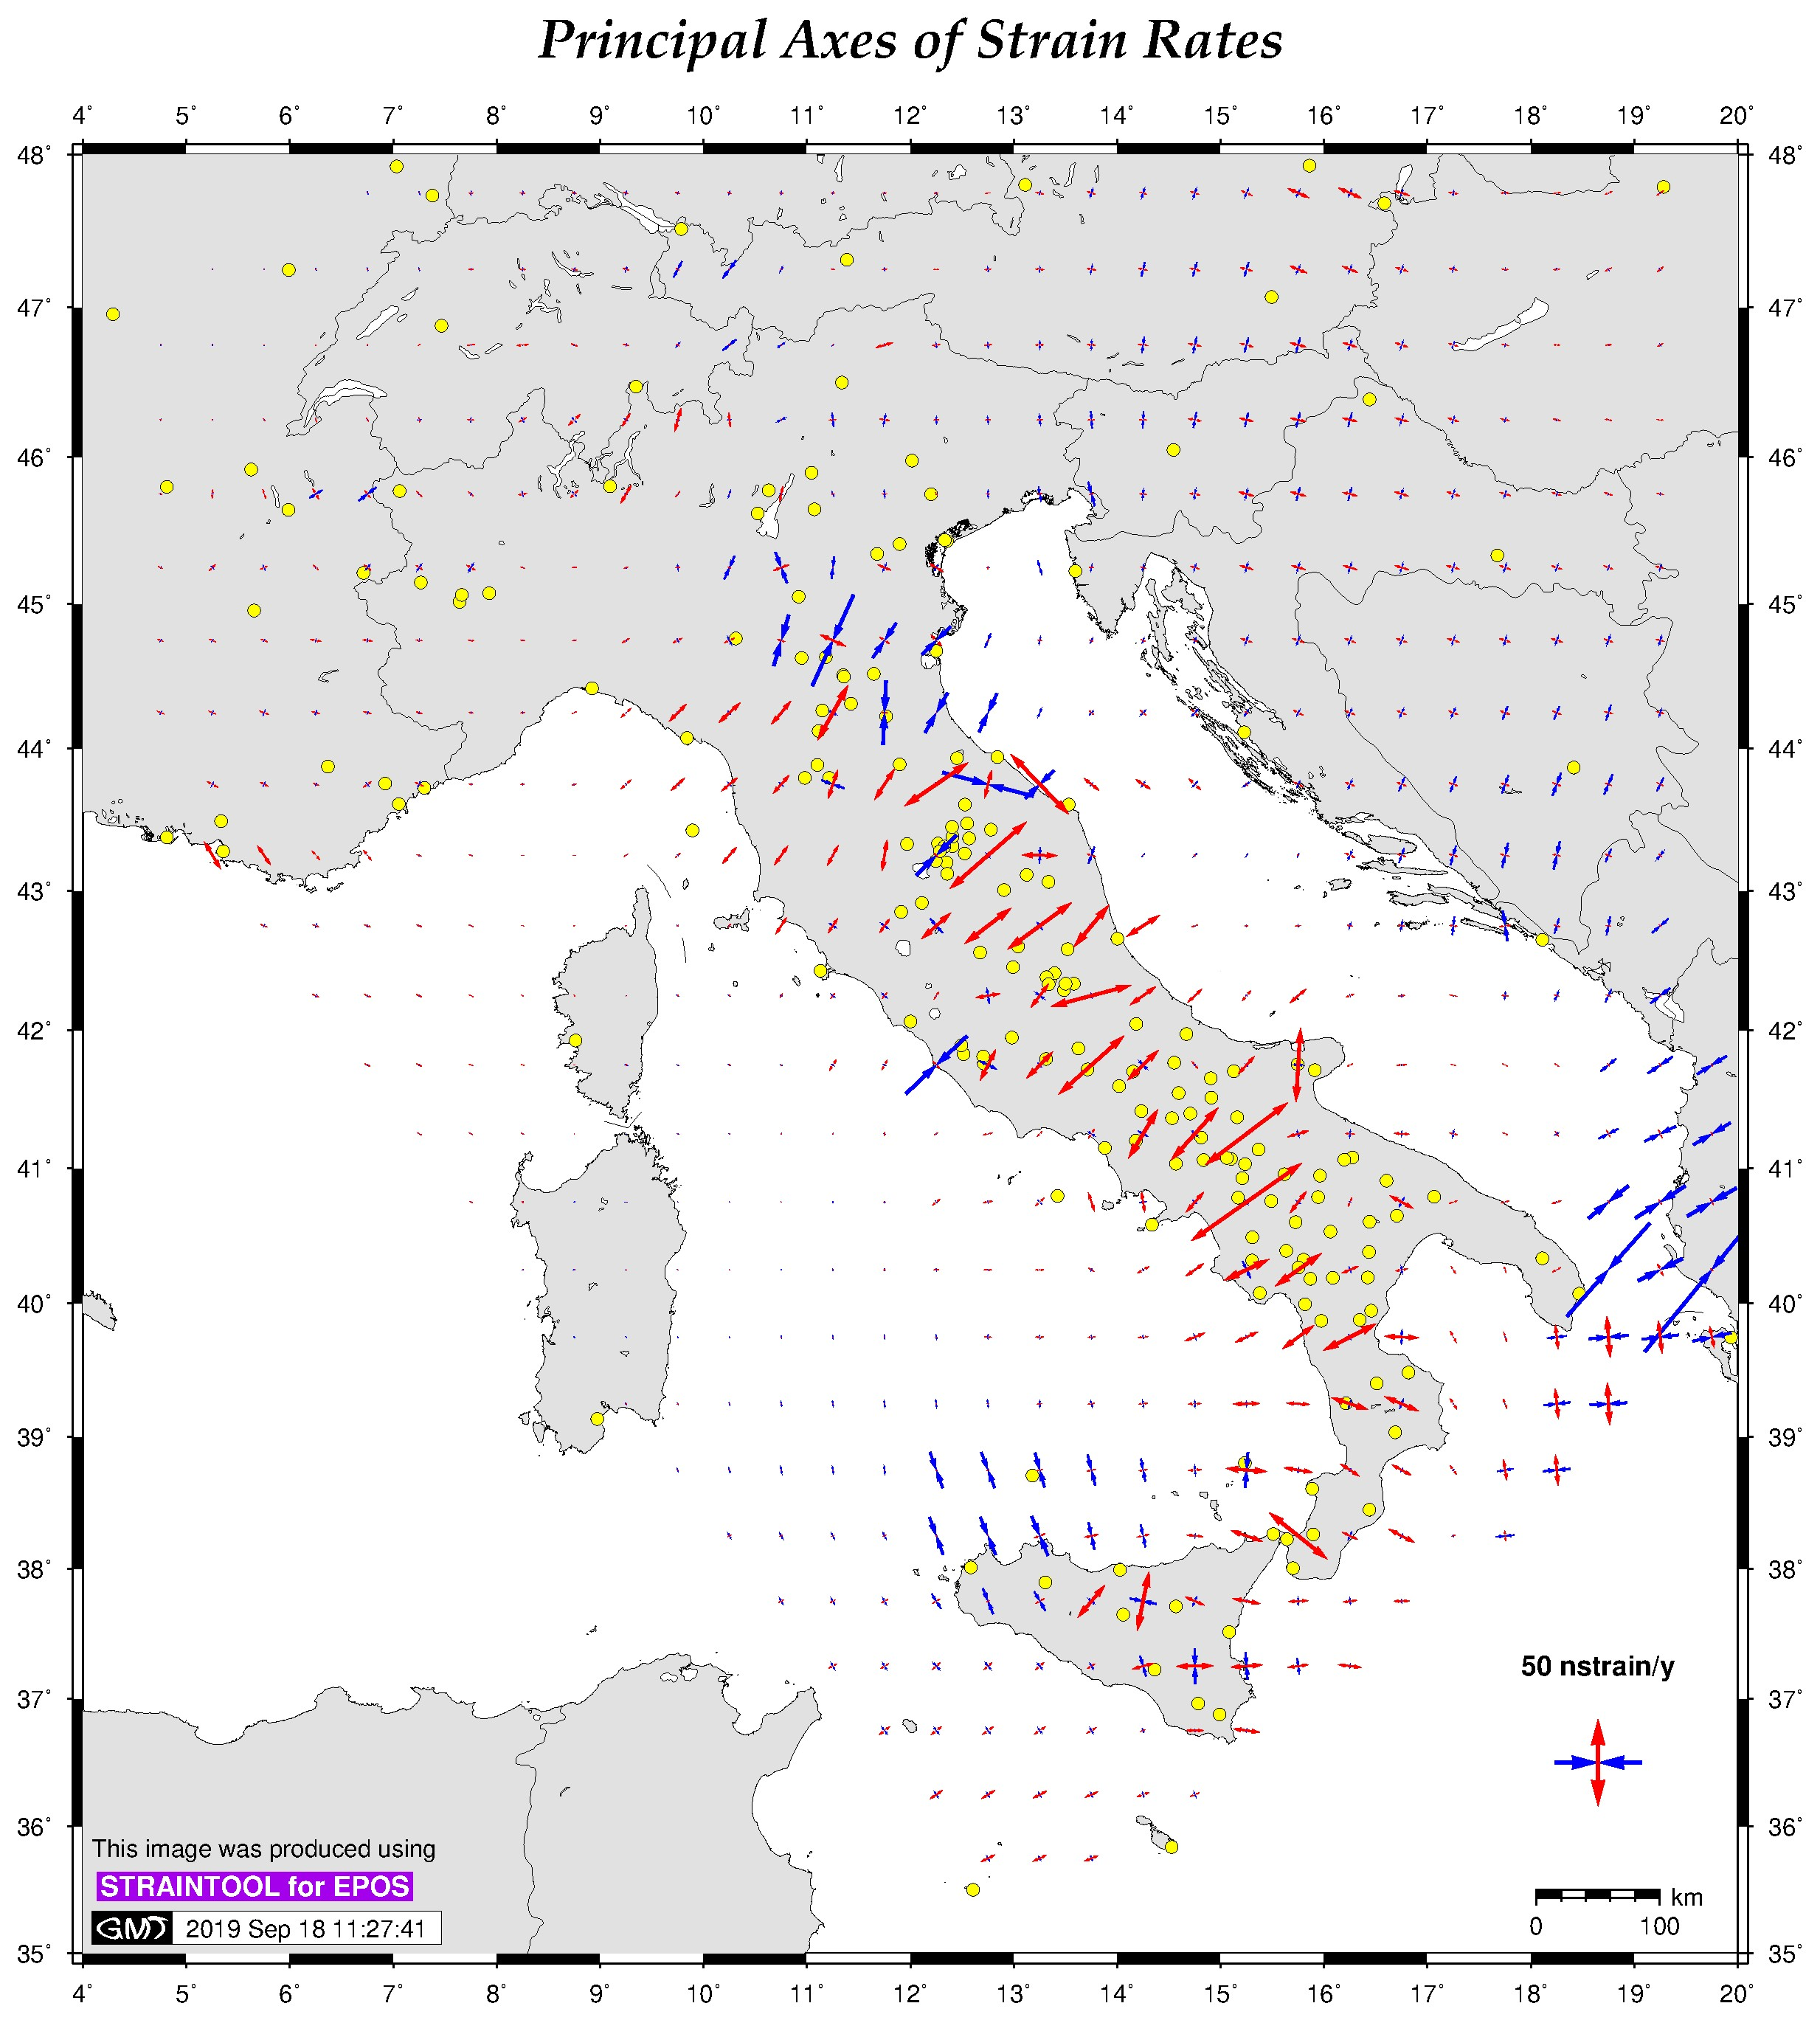
\includegraphics[width=.95\textwidth]{itmidas-output_str.jpg}
      \end{center}
    \end{column}
    \begin{column}{0.58\textwidth}
      \begin{center}
        \citet{DAgostino2014}
        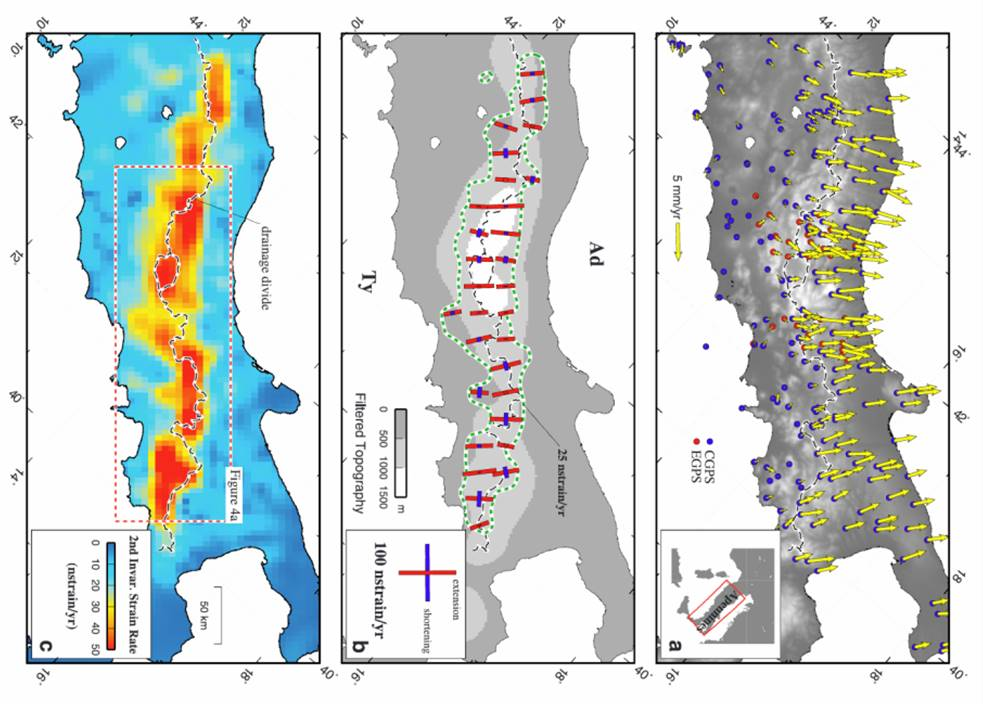
\includegraphics[width=0.95\textwidth]{dagostino_italy.jpg}     
      \end{center}
    \end{column}
  \end{columns}

\end{frame}
\note{}

\begin{frame}
  \frametitle{Strain Analysis}
  \framesubtitle{Italy region}
  \label{ch4:}

  \begin{columns}
    \begin{column}{0.5\textwidth}
      \begin{center}
        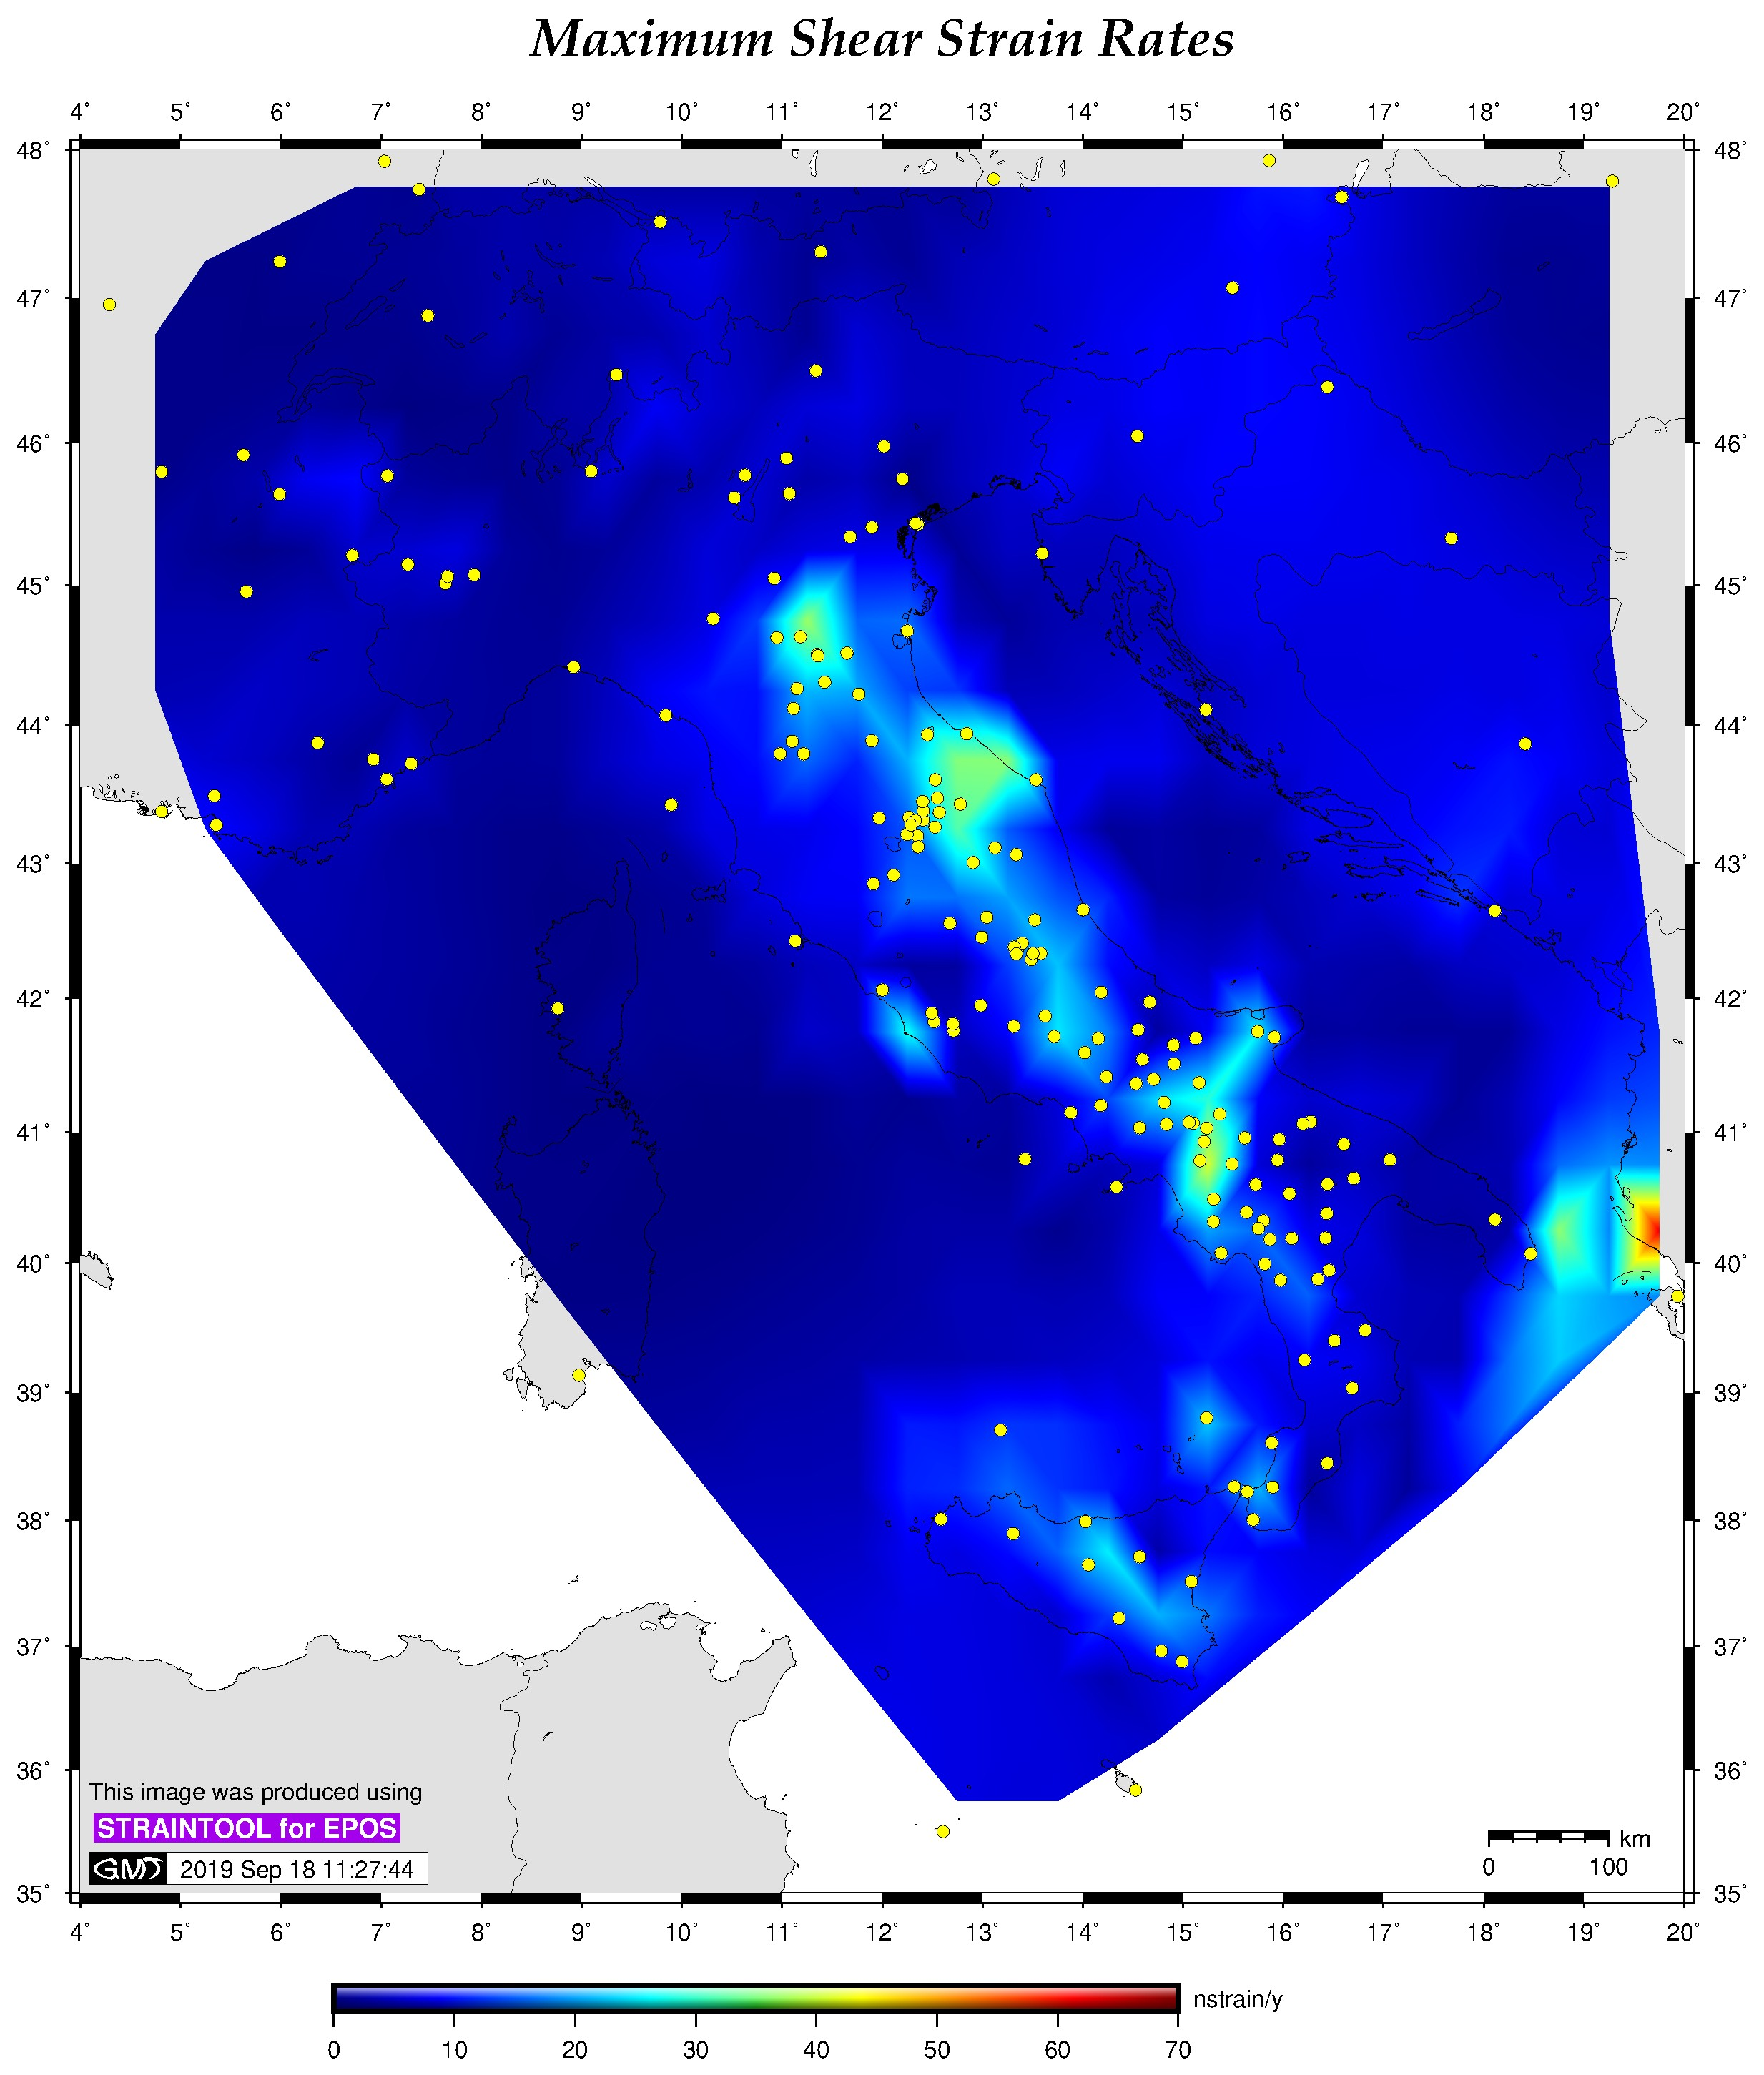
\includegraphics[width=.98\textwidth]{itmidas-output_gtot.jpg}   
      \end{center}
    \end{column}
    \begin{column}{0.5\textwidth}
      \begin{center}
        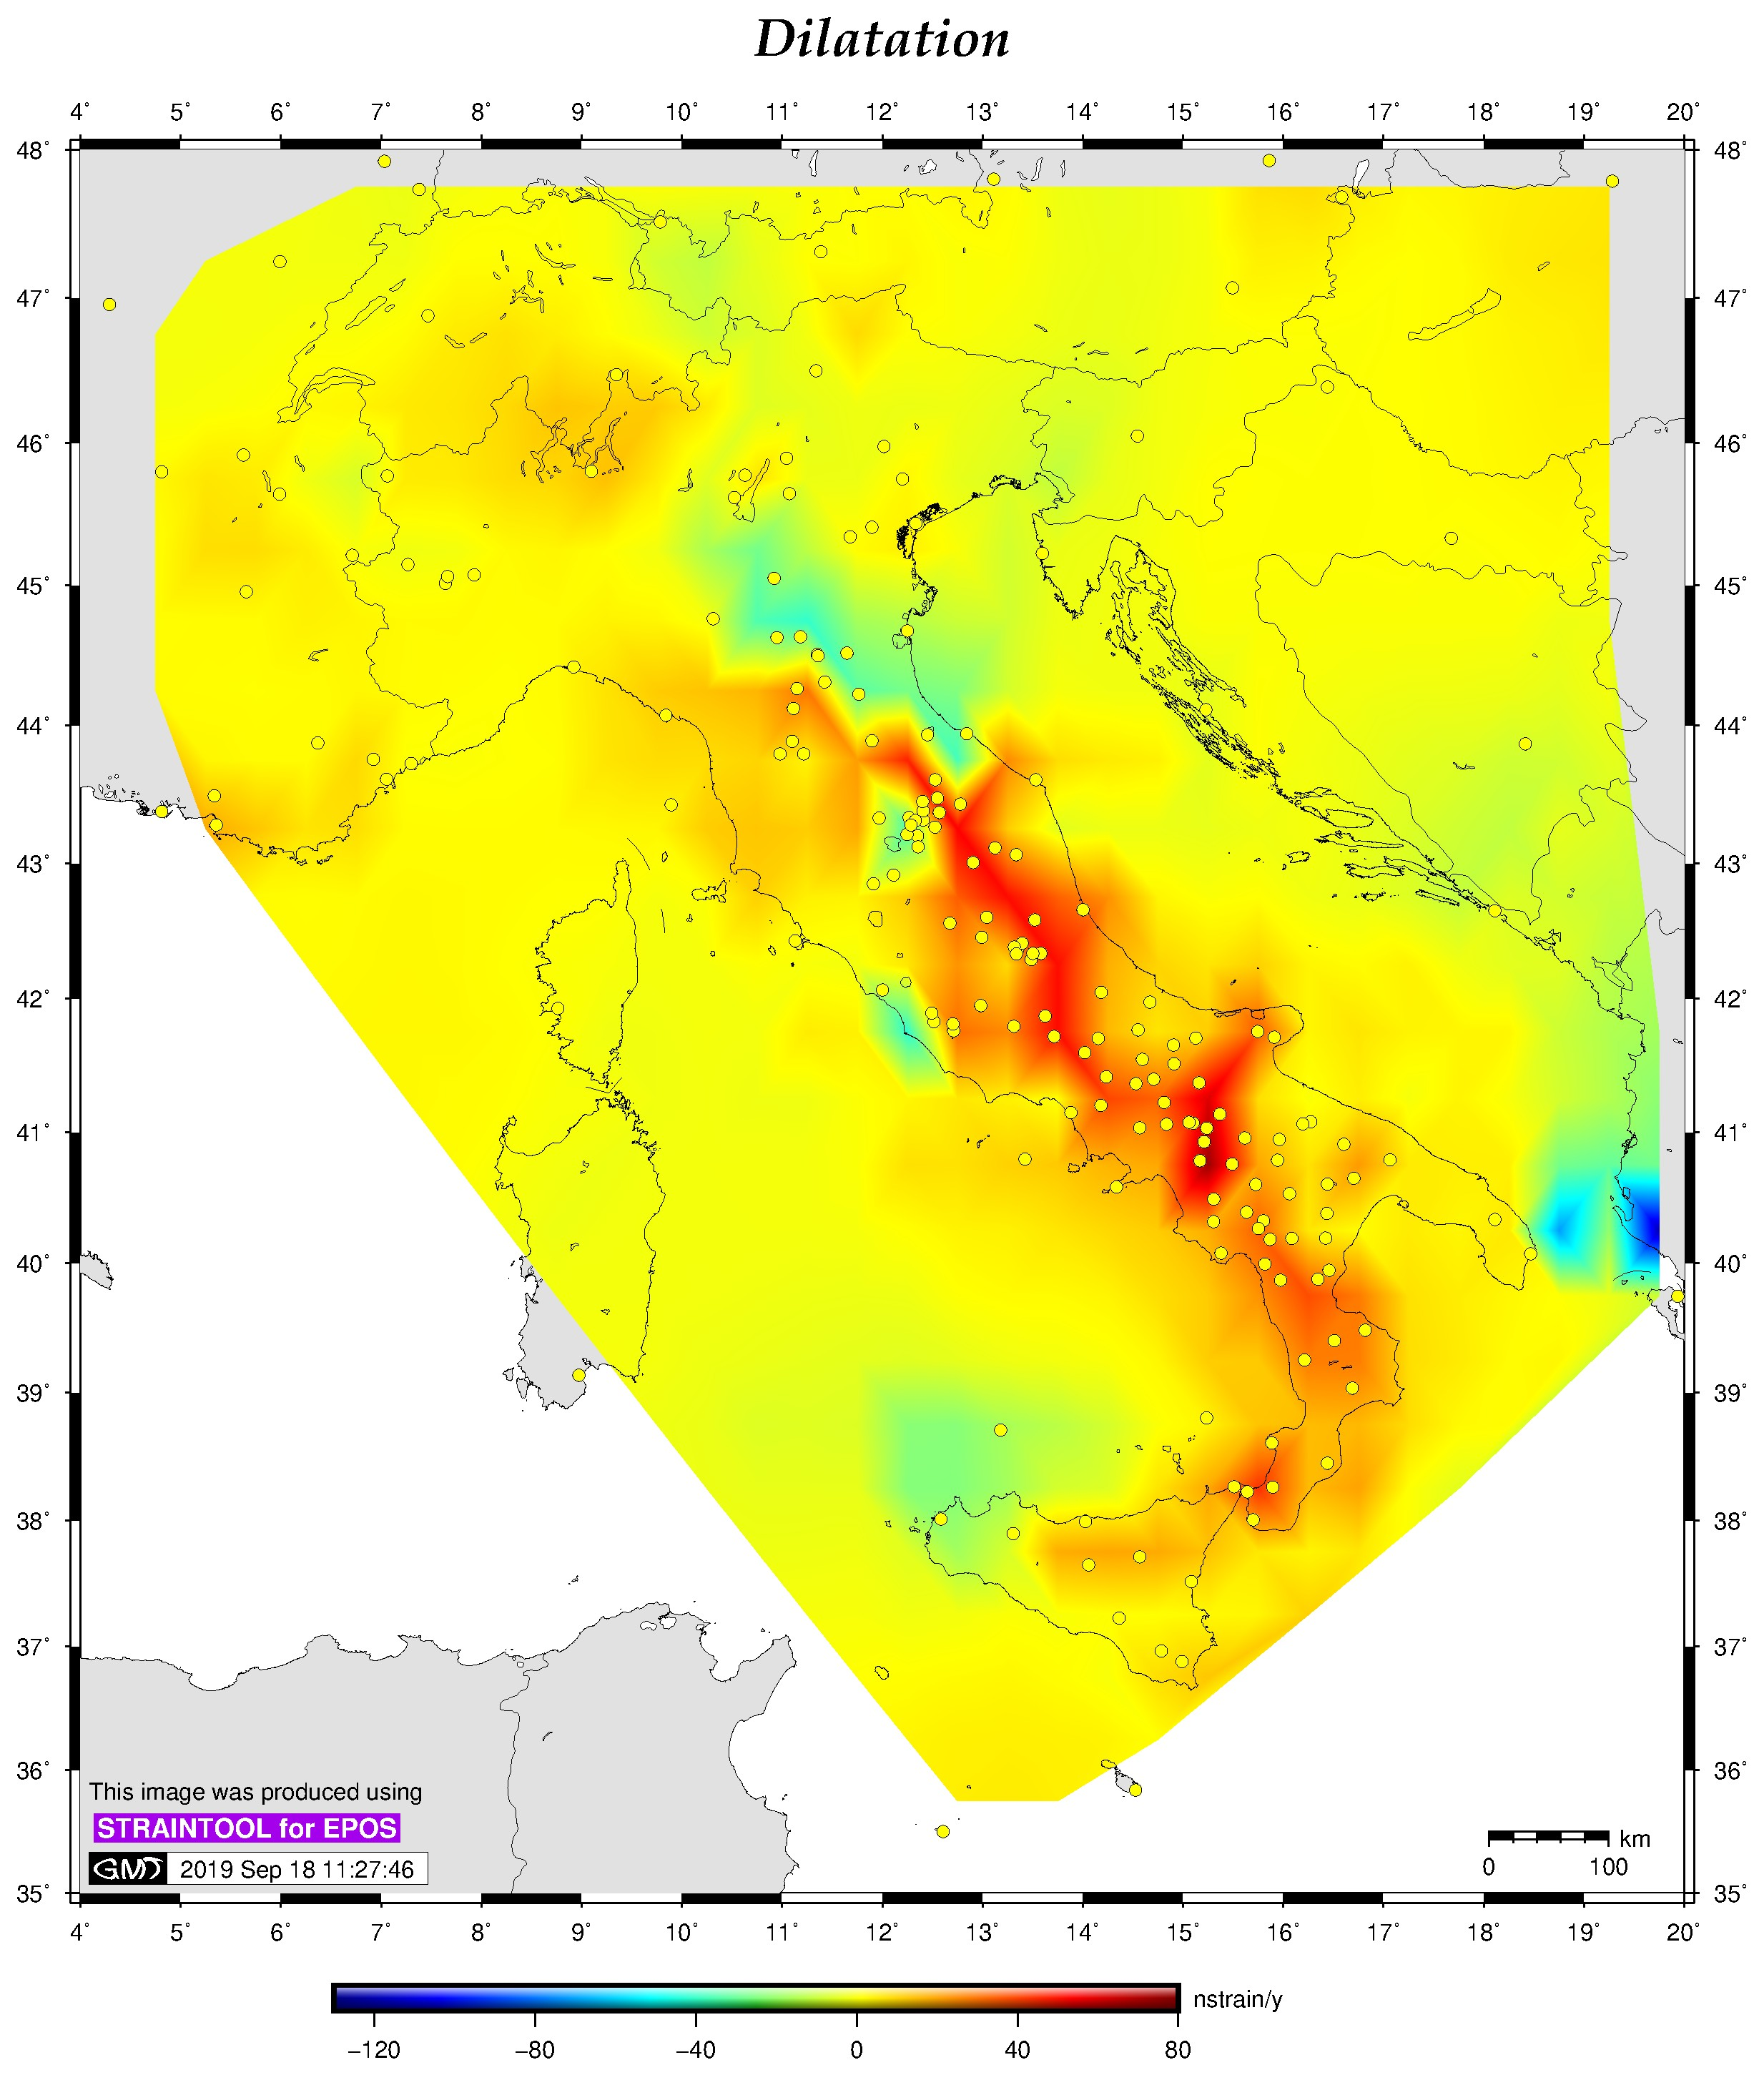
\includegraphics[width=0.98\textwidth]{itmidas-output_dil.jpg}     
      \end{center}
    \end{column}
  \end{columns}

\end{frame}
\note{}

\begin{frame}
  \frametitle{Statistics}
  \framesubtitle{Sigma value}
  \label{ch4:}
   
  \begin{columns}
    \begin{column}{0.5\textwidth}
      \begin{center}
        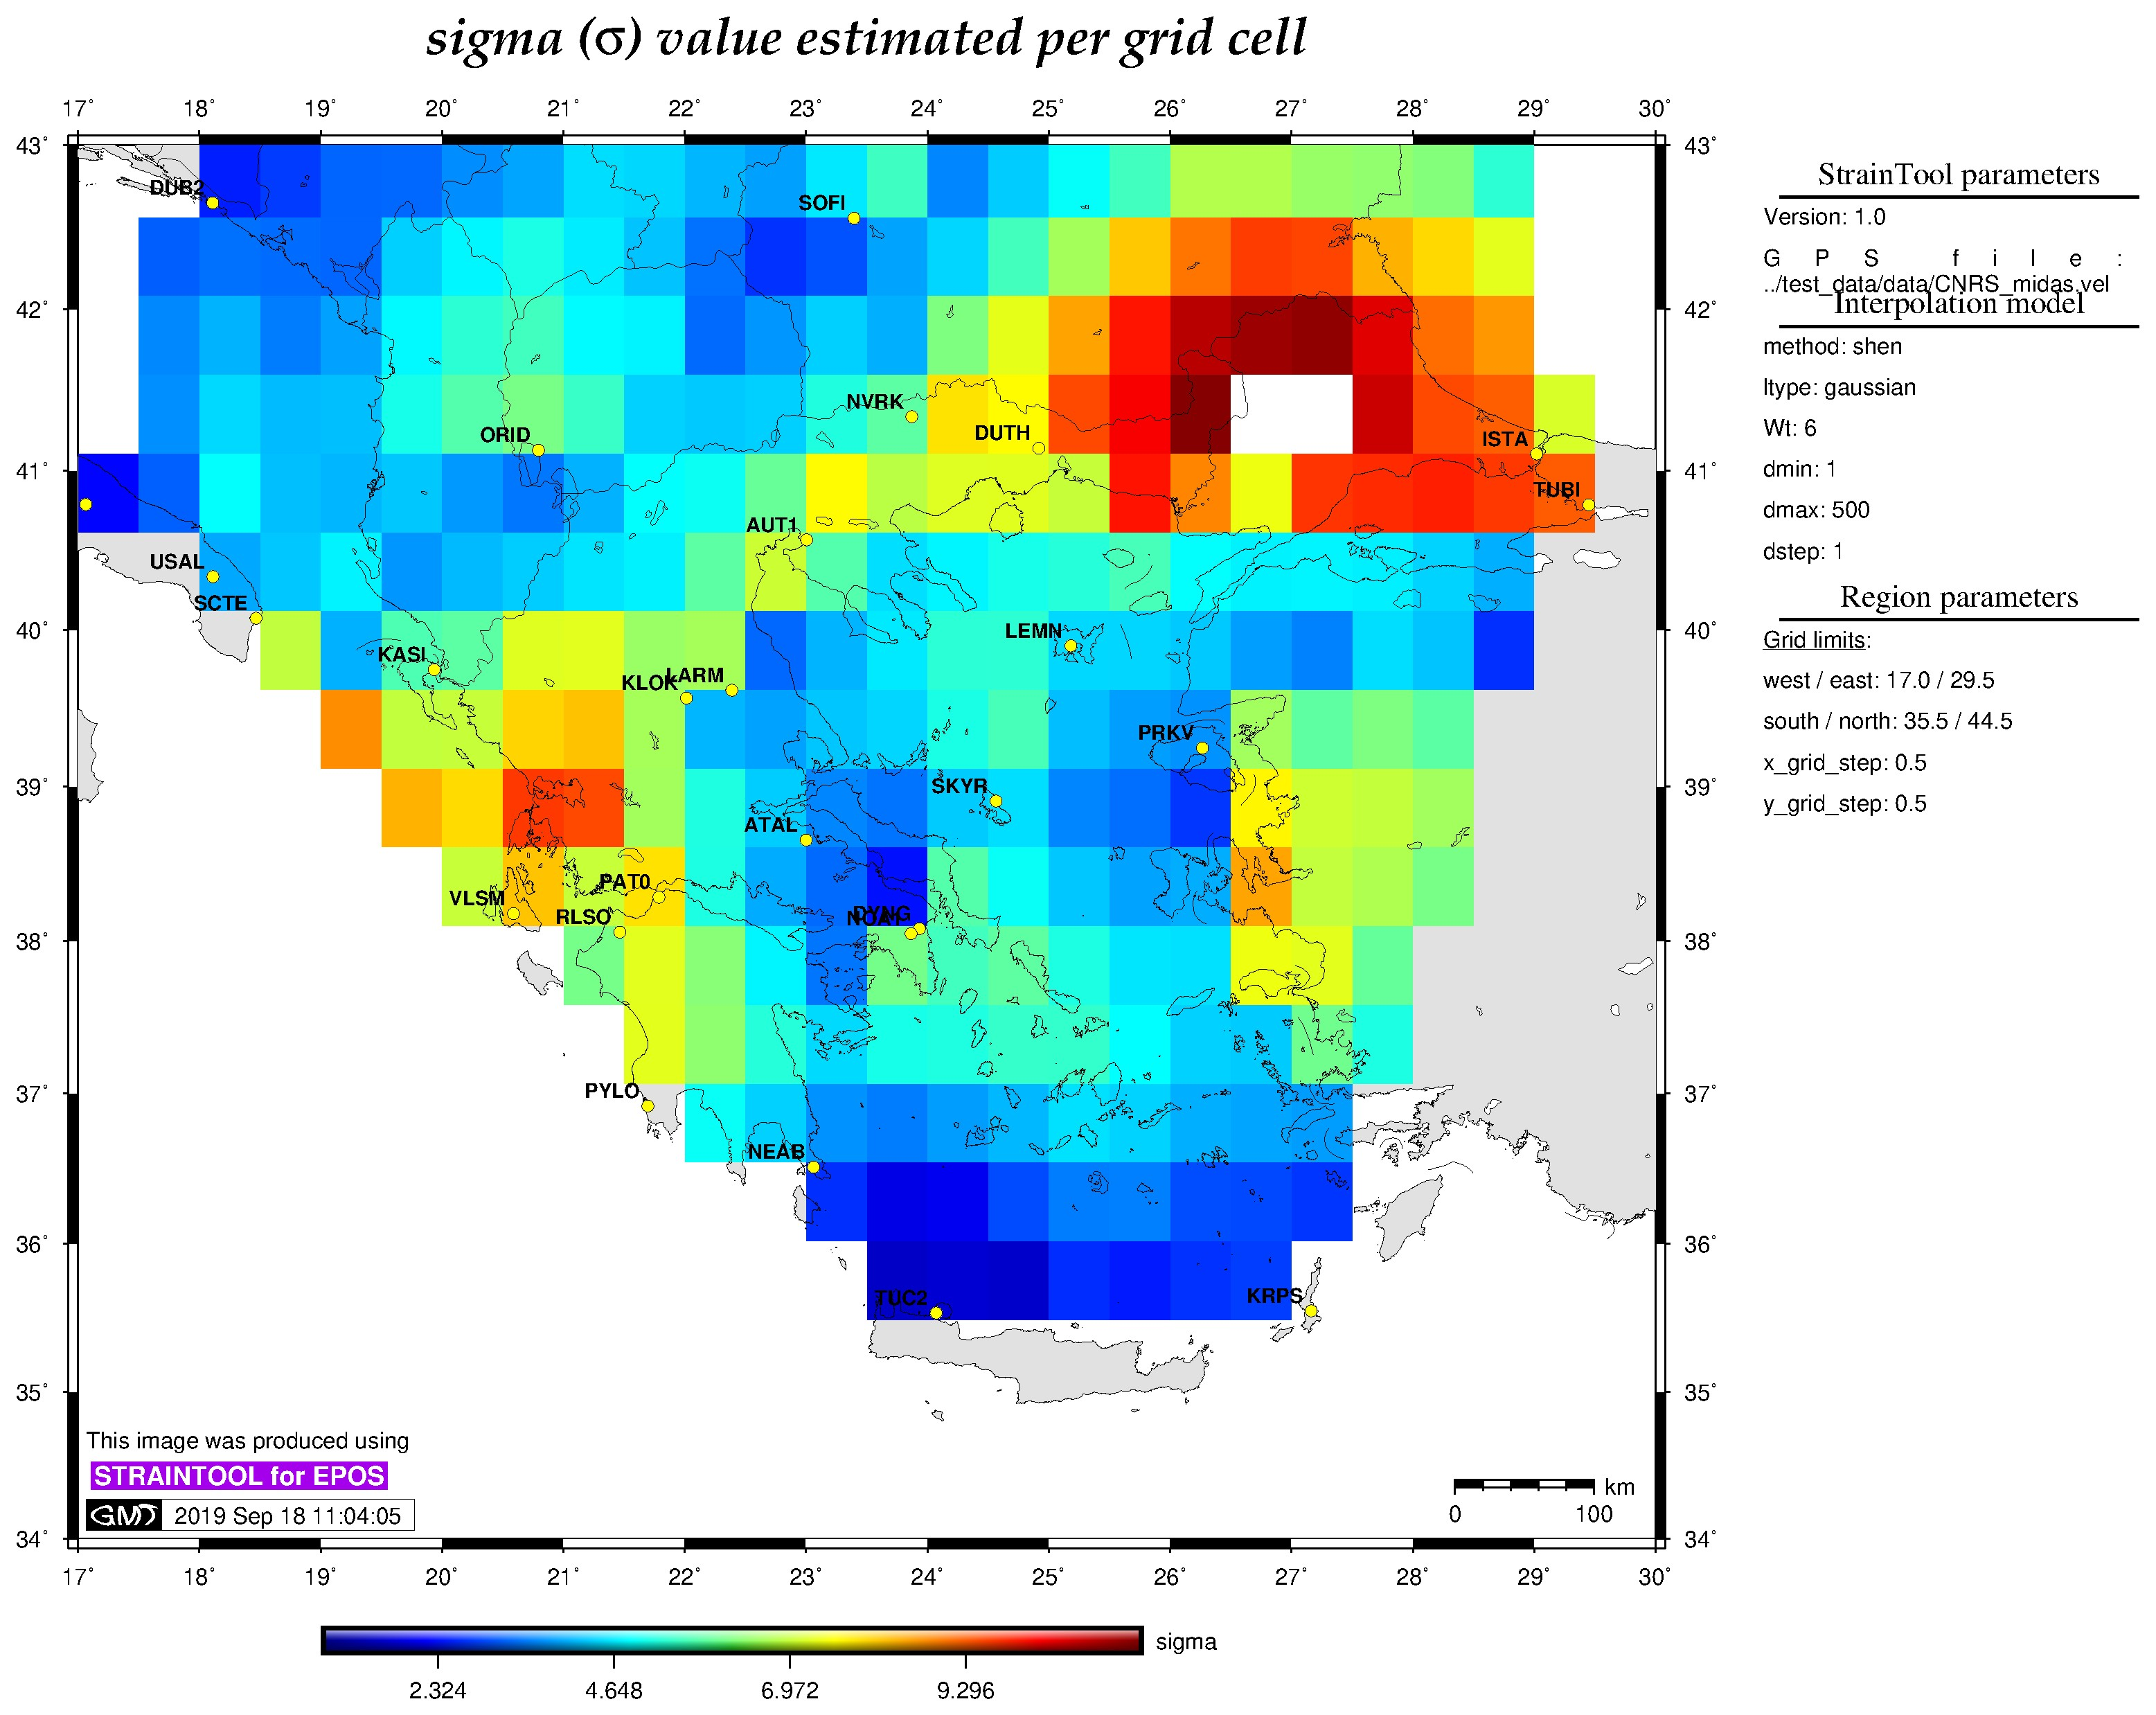
\includegraphics[width=.98\textwidth]{grmidas-output_stats-sigma.jpg}   
      \end{center}
    \end{column}
    \begin{column}{0.5\textwidth}
      \begin{center}
        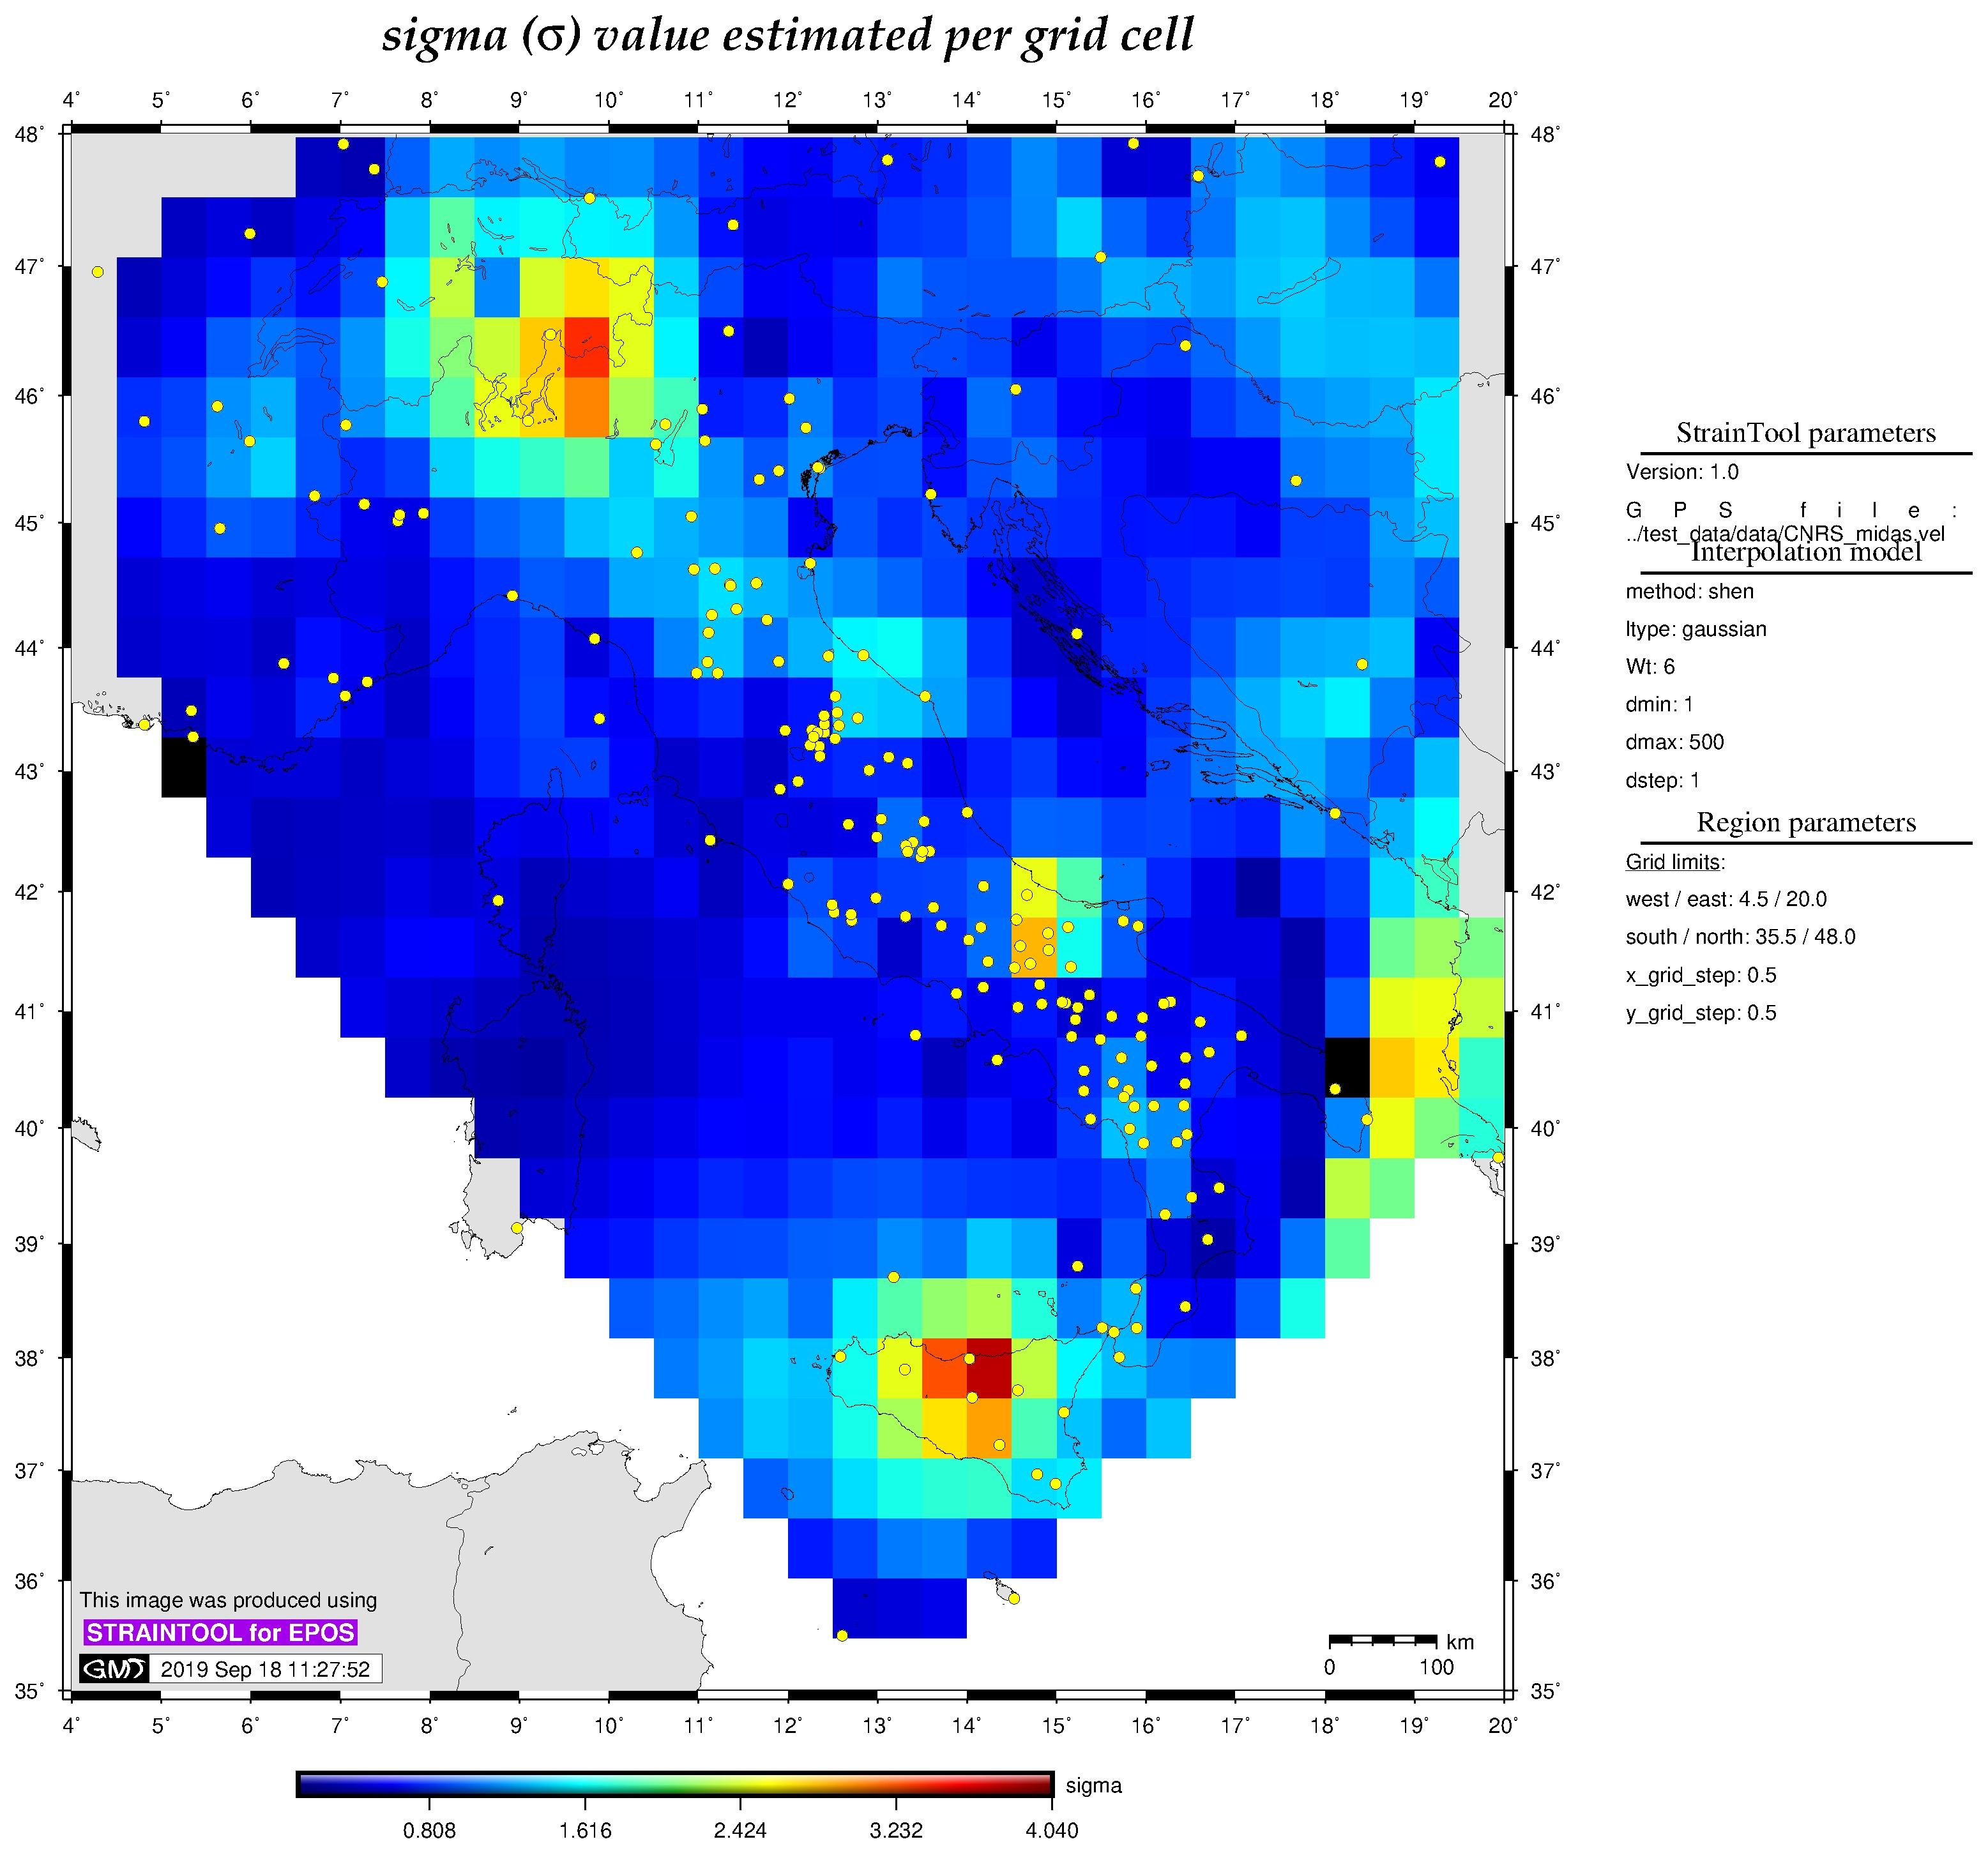
\includegraphics[width=0.98\textwidth]{itmidas-output_stats-sigma.jpg}     
      \end{center}
    \end{column}
  \end{columns}

\end{frame}
\note{}

\begin{frame}
  \frametitle{Statistics}
  \framesubtitle{D optimal smoothing parameter}
  \label{ch4:}
   
  \begin{columns}
    \begin{column}{0.5\textwidth}
      \begin{center}
        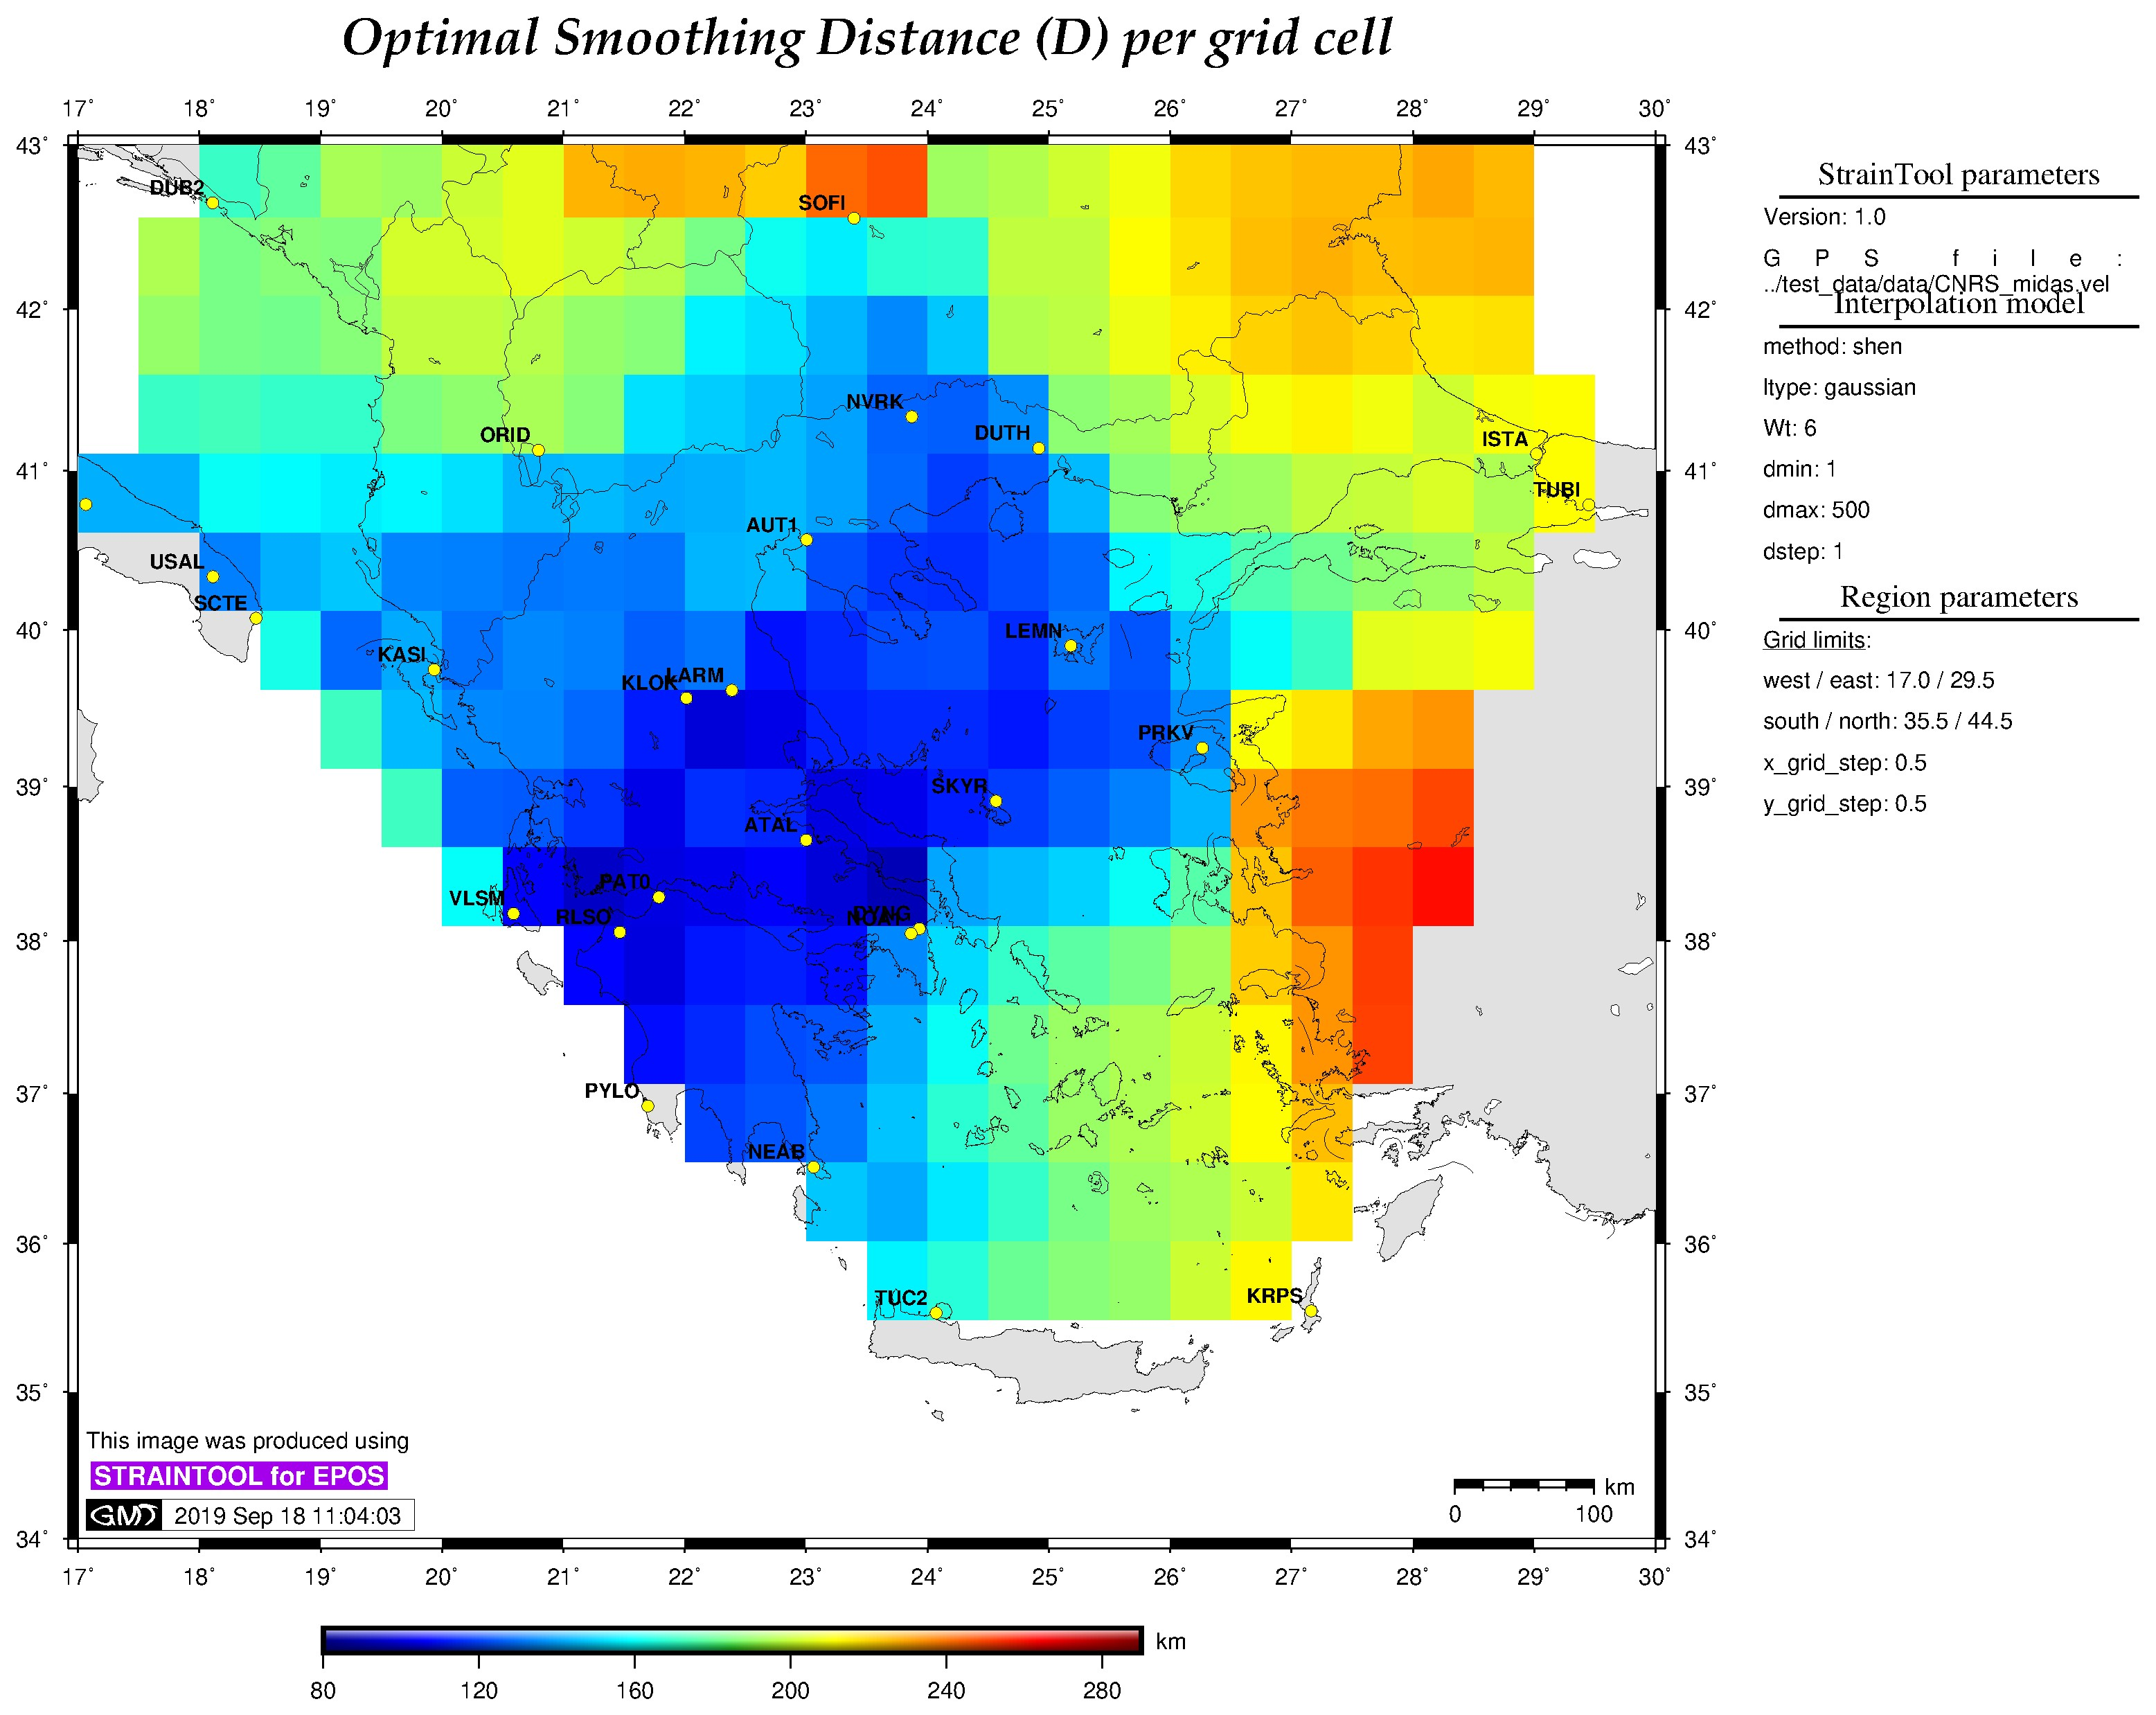
\includegraphics[width=.98\textwidth]{grmidas-output_stats-doptimal.jpg}   
      \end{center}
    \end{column}
    \begin{column}{0.5\textwidth}
      \begin{center}
        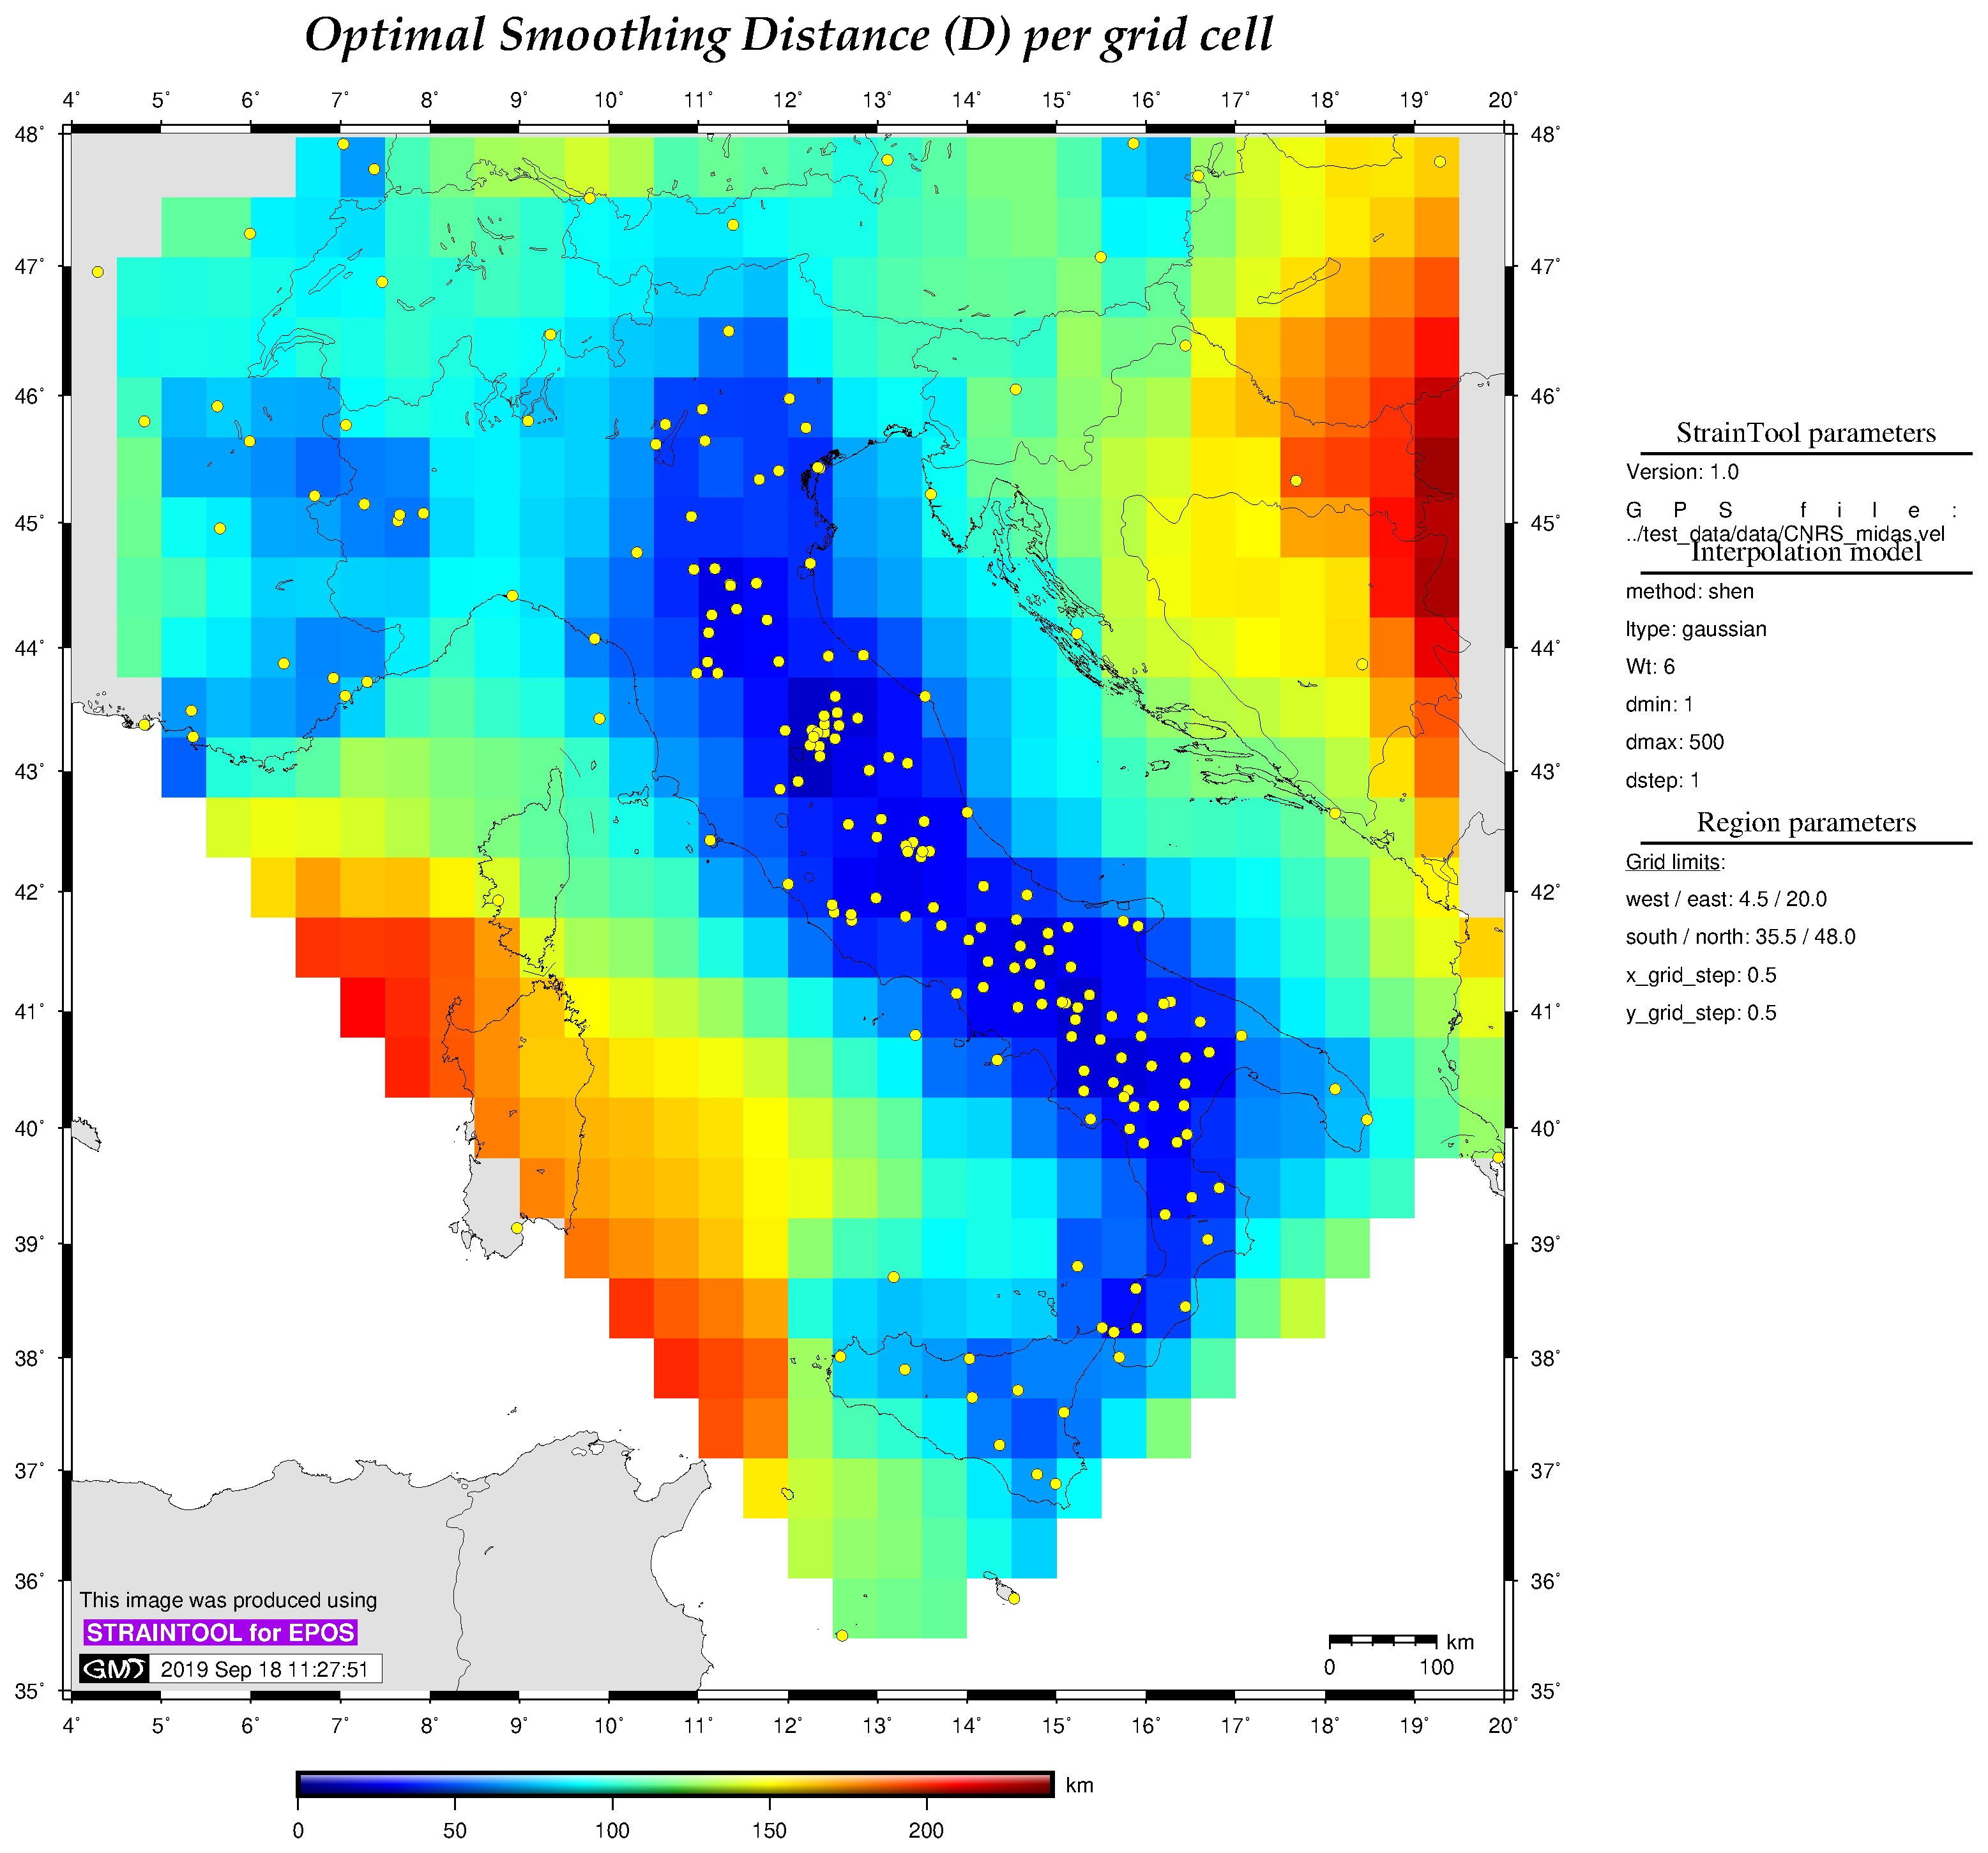
\includegraphics[width=0.98\textwidth]{itmidas-output_stats-doptimal.jpg}     
      \end{center}
    \end{column}
  \end{columns}

\end{frame}
\note{}

%\begin{frame}
%  \frametitle{}
%  \framesubtitle{}
%  \label{ch4:}

%\end{frame}
%\note{}
